\section{Supplementary results}
\label{sec:result_balibase}

\subsection{Dataset statistics}
\label{sec:dataset_stat}
% Table generated by Excel2LaTeX from sheet 'Sheet1'
\subsubsection{100-taxon simulated dataset}
We used five randomly selected replicates (R0, R4, R9, R14, R19) of simulated nucleotide dataset from the study of~\citealp{liu2009rapid}. It is publicly available at \url{https://sites.google.com/eng.ucsd.edu/datasets/sate-i}. Table~\ref{tab:sim_stat} gives the reference alignment statistics for this dataset.

\begin{table}[htbp]
	\centering
	\caption{Reference alignments for 100-taxon simulated dataset.}
	\begin{tabular}{|l|r|}
		\hline
		\multicolumn{1}{|c|}{Feature} & \multicolumn{1}{c|}{Value} \\
		\hline
		Number of taxa & 100 \\
		\hline
		Number of sites & 1698.2 \\
		\hline
		Percent indels & 40.4 \\
		\hline
		Avg. gap length & 3.1 \\
		\hline
	\end{tabular}%
	\label{tab:sim_stat}%
\end{table}%


\subsubsection{Biological rRNA datasets}
We analyzed two biological ribosomal RNA datasets, 23S.E and 23S.E.aa\_ag, from~\citealp{liu2009rapid} which are challenging for phylogeny estimation methods. Each of these datasets is given with a highly reliable, curated reference alignment from Gutell Lab. The statistics of the reference alignments of these datasets are presented in Table~\ref{tab:bio_stat}. Reference trees for these datasets were generated from the reference alignments by running RAxML~\citep{stamatakis2014raxml} with bootstrapping, and retaining only the highly supported edges. We evaluated generated alignments with respect to the reference alignment using the tool FastSP \citep{mirarab2011fastsp}.
% Table generated by Excel2LaTeX from sheet 'Sheet2'
\begin{table}[htbp]
	\small
	\centering
	\caption{Reference alignments for two biological rRNA datasets.}
	\begin{tabular}{|l|r|r|}
		\hline
		\multicolumn{1}{|c|}{Feature} & \multicolumn{1}{c|}{23S.E.aa\_ag} & \multicolumn{1}{c|}{23S.E} \\
		\hline
		Number of taxa & 144   & 117 \\
		\hline
		Number of sites & 8,619 & 9,079 \\
		\hline
		Percent indels & 61.1  & 59.7 \\
		\hline
		Avg. gap length & 13.5  & 12.6 \\
		\hline
	\end{tabular}%
	\label{tab:bio_stat}%
\end{table}%

\subsubsection{BAliBASE datasets}
BAliBASE 3.0 \citep{thompson2005balibase} is the most widely used benchmark alignment databases of protein families. It provides manually refined reference alignments of high quality based on 3D structural superposition. These datasets are organized into six groups according to their families and similarities: RV11 (very divergent sequences, residue identity below 20\% ), RV12 (medium to divergent sequences, 20\%-40\% residue identity), RV20 (families with one or more highly divergent sequences), RV30 (divergent subfamilies), RV40 (sequences with large terminal N/C extensions), and RV50 (sequences with large internal insertions). In this study, we selected four to five representative datasets from each group as reported in Table~\ref{tab:balibase}. We generated reference trees for these datasets by running RAxML~\citep{stamatakis2014raxml} with bootstrapping. We evaluated estimated alignments with respect to the core blocks (regions for which reliable alignments are known to exist) using the program bali\_score available at~\url{http://www.lbgi.fr/balibase/BalibaseDownload/}.

% Table generated by Excel2LaTeX from sheet 'Sheet2'
\begin{table}[htbp]
	\small
	\centering
	\caption{ BAliBASE datasets selected for this study.}
	\begin{tabular}{|l|l|}
		\hline
		\multicolumn{1}{|c|}{Group} & \multicolumn{1}{c|}{Datasets selected} \\
		\hline
		RV11  & BB11005, BB11018, BB11020, BB11033 \\
		\hline
		RV12  & BB12001, BB12013, BB12022, BB12035, BB12044 \\
		\hline
		RV20  & BB20001, BB20010, BB20022, BB20033, BB20041 \\
		\hline
		RV30  & BB30002, BB30008, BB30015, BB30022 \\
		\hline
		RV40  & BB40001, BB40013, BB40025, BB40038, BB40048 \\ %
		\hline
		RV50  & BB50001, BB50005, BB50010, BB50016 \\
		\hline
	\end{tabular}%
	\label{tab:balibase}%
\end{table}%

\subsection{Selection of appropriate multi-objective formulations}
\textit{(The following should be read in conjunction with the description presented in Section~\ref{sec:selection_msa_formulation} of the main text)} 

We visualize the interrelations among the objective values of the solutions, obtained by running NSGA-III to optimizes the objective set \{Gap, SOP, wSOP, TC\} on five randomly selected replicates (R0, R4, R9, R14, R19) of 100-taxon simulated dataset, using a $ 4\times4 $ scatter-plot matrix~\cite{kalyanmoy2001multi} as shown in Figure~\ref{fig:nature_obj}. Here each diagonal cell of a matrix depicts the distribution of the values of an objective function estimated using kernel density estimation which is a non-parametric way to estimate the probability density function of a random variable. And the non-diagonal cells show the correlation between each pair of objective functions. As our evolutionary algorithms tries to minimize all objective functions, we treat the maximization objective values by multiplying with -1. In the sequel, we normalize all the objective values using min-max technique and as such the maximization objectives are turned into minimization ones.

We estimate the coefficients of multiple linear regression model associating FN rate with each of the objective function from \{Gap, SOP, wSOP, TC\} using least-squares method and illustrate them using partial regression plots~\citep{montgomery2012introduction} in Figure~\ref{fig:mul_lin_reg}. We apply $t$-test on individual regression coefficient (i.e., slope) $\beta_i$ (with null hypothesis $\beta_i=0$) to test the significance of that association. The test results (slope, $p$-value) are incorporated in the figure.

We measure the strength of each objective set based on the FN rate achieved by the members of generated solution set. To accomplish this, For each set of objective functions, we run NSGA-II~\citep{deb2002fast} for 20 times following the standard practice of operations research (OR) literature (due to the stochastic nature of metaheuristics). Each run generates a set of solutions that represents the trade-offs in satisfying all objectives. Afterwards, we inferred ML tree for each of the generated alignment. We collected the best FN rates from each of the 20 solution sets and describe the distribution of these FN rates using boxplots which are shown in Figure~\ref{fig:rank_best_fn_rate}. In these boxplots we also incorporate the FN rates achieved by the state-of-the-art tools for comparison using horizontal lines.

\begin{figure*}[!htbp]	
	\begin{adjustwidth}{-1cm}{-1cm}
		\centering
		\begin{subfigure}{0.35\textwidth}
			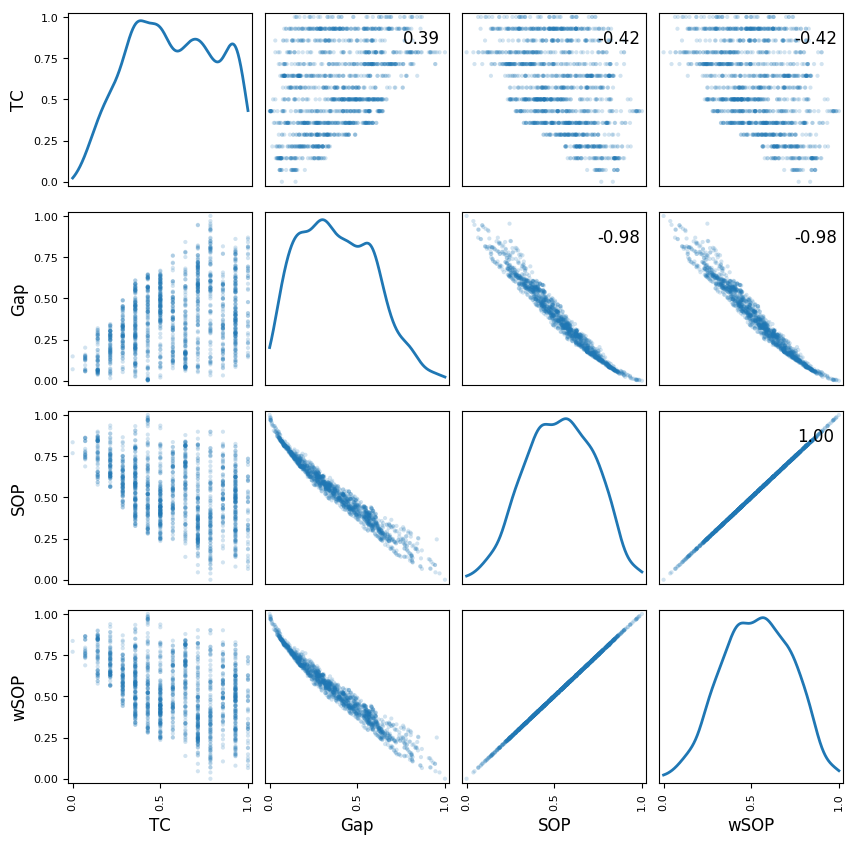
\includegraphics[width=\columnwidth]{Figure/NumGaps_SOP_TC_wSOP/precomputedInit/R0/fig/scatter_mattrix}
			\caption{R0}
			%\label{fig:con_pr09}
		\end{subfigure}	
		\begin{subfigure}{0.35\textwidth}
			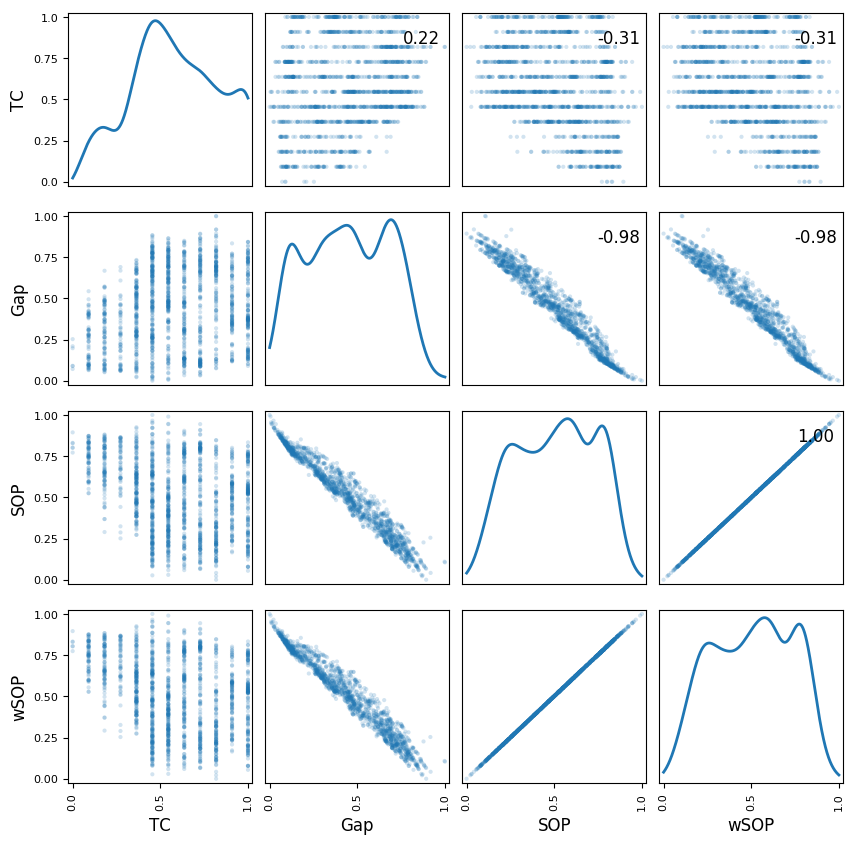
\includegraphics[width=\columnwidth]{Figure/NumGaps_SOP_TC_wSOP/precomputedInit/R4/fig/scatter_mattrix}
			\caption{R4}
			%\label{fig:con_pr09}
		\end{subfigure}
		\begin{subfigure}{0.35\textwidth}
			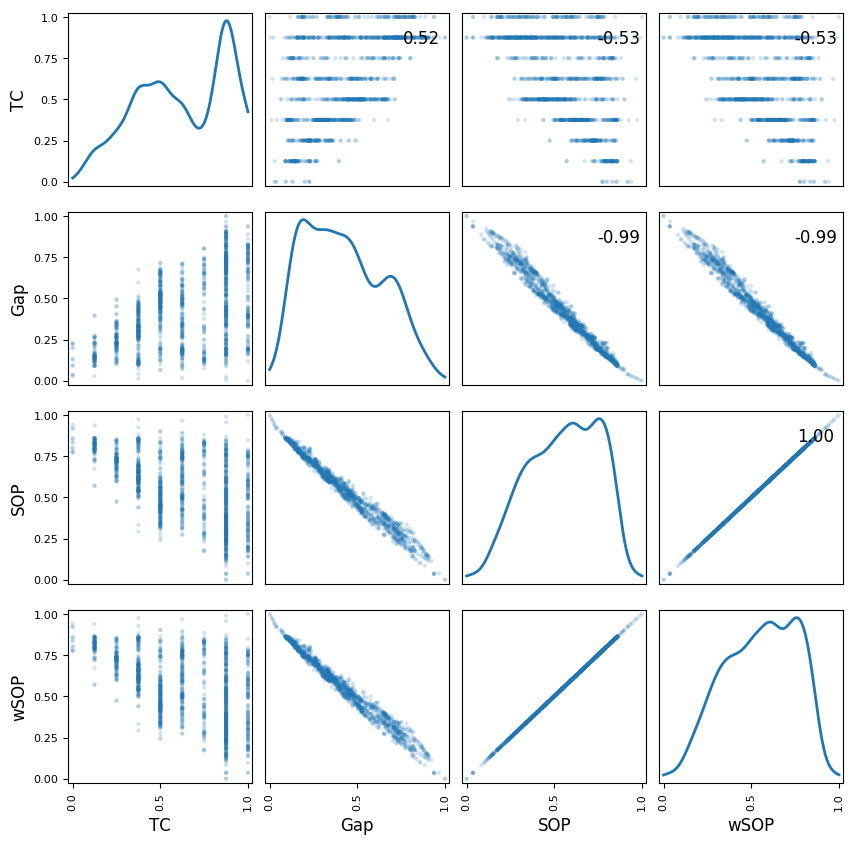
\includegraphics[width=\columnwidth]{Figure/NumGaps_SOP_TC_wSOP/precomputedInit/R9/fig/scatter_mattrix}
			\caption{R9}
			%\label{fig:con_pr09}
		\end{subfigure}
		\begin{subfigure}{0.35\textwidth}
			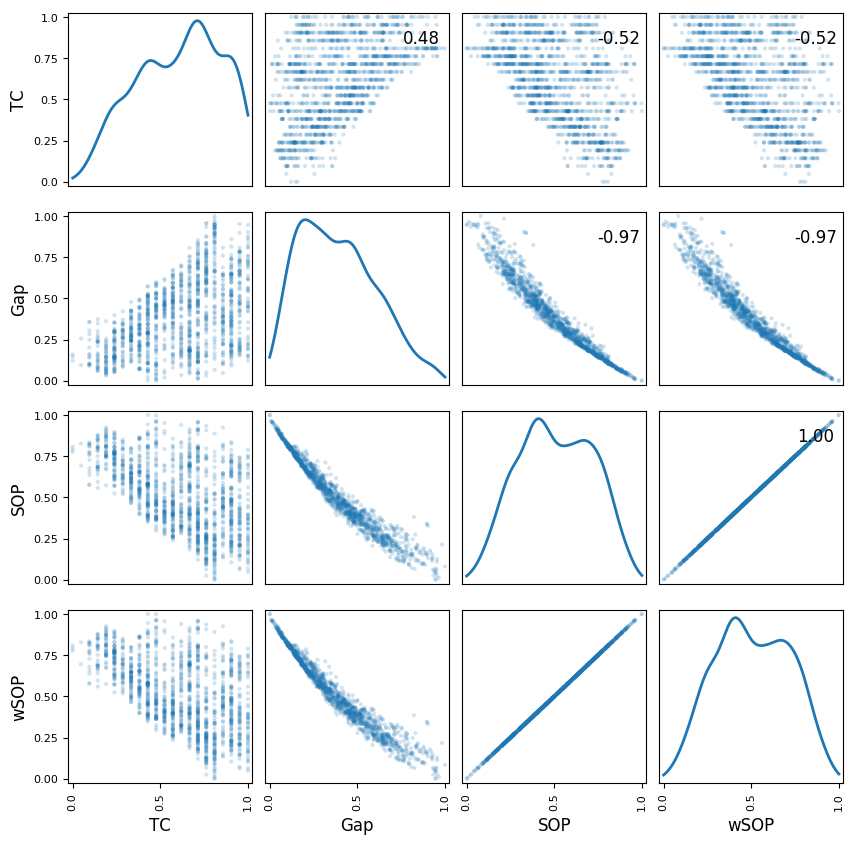
\includegraphics[width=\columnwidth]{Figure/NumGaps_SOP_TC_wSOP/precomputedInit/R14/fig/scatter_mattrix}
			\caption{R14}
			%\label{fig:con_pr09}
		\end{subfigure}
		\begin{subfigure}{0.35\textwidth}
			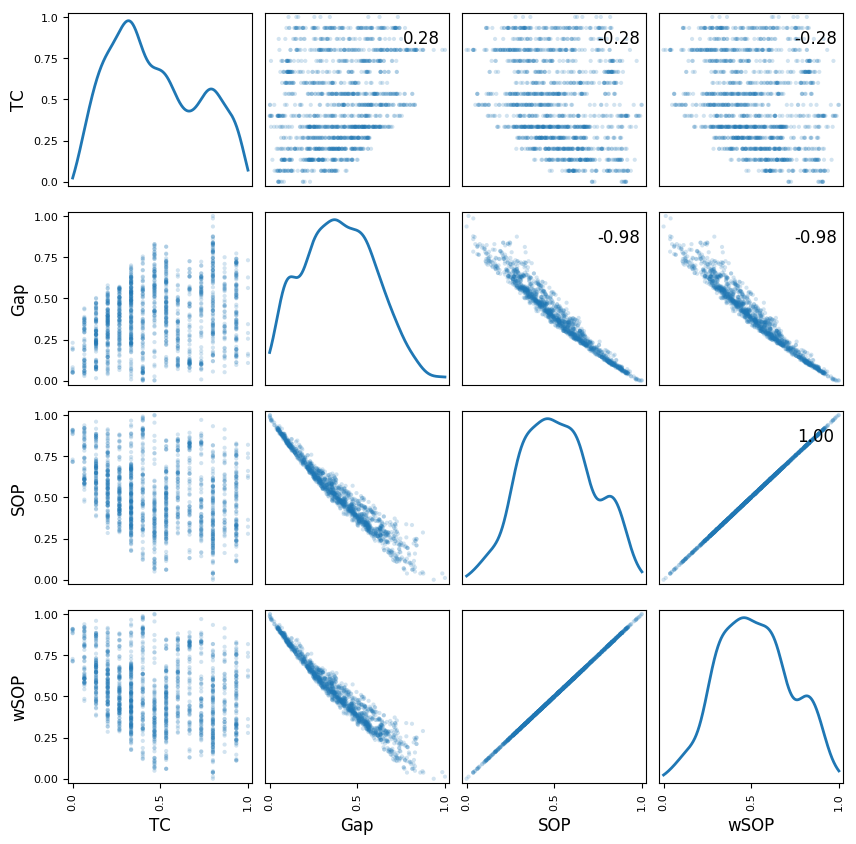
\includegraphics[width=\columnwidth]{Figure/NumGaps_SOP_TC_wSOP/precomputedInit/R19/fig/scatter_mattrix}
			\caption{R19}
			%\label{fig:con_pr09}
		\end{subfigure}
		\caption{\underline{100-taxon simulated dataset:} Scatter-plot matrices depicting the pairwise relationship of all objective functions on five randomly selected replicates. We turn each objective function into minimization form and then normalize using min-max technique. In each matrix, the diagonal cells show the distribution of objective values (estimated using kernel density estimation which is a non-parametric way to estimate the probability density function of a random variable) while the non-diagonal cells show the correlation between pairs of objective functions. Each upper-diagonal cell contains the value of correlation coefficient $r$ of the corresponding pair of objective functions.}
		\label{fig:nature_obj}
	\end{adjustwidth}
\end{figure*}

\begin{figure*}[!htbp]
	\centering
	\small
	\begin{adjustwidth}{-1cm}{-1cm}
		\begin{tabular}{l||C{0.24\textwidth}|C{0.24\textwidth}|C{0.24\textwidth}|C{0.24\textwidth} }
			& TC & Gap & SOP & wSOP\\\hline\hline
			\rotatebox[origin=c]{-90}{R0} & 
			\raisebox{-.5\height}{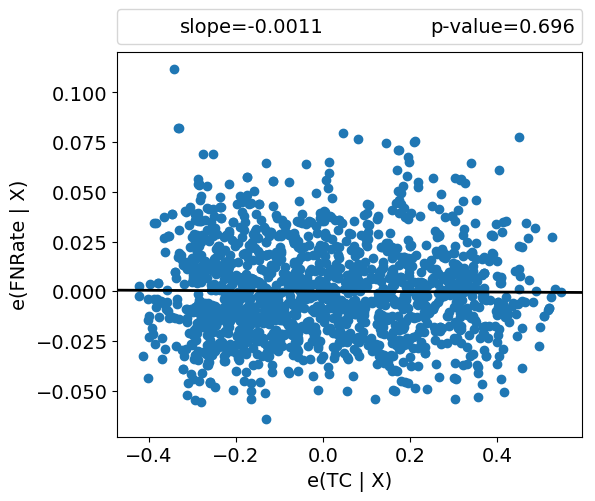
\includegraphics[width=0.25\textwidth]{Figure/NumGaps_SOP_TC_wSOP/precomputedInit/R0/fig/tc_partial_regression}} &
			\raisebox{-.5\height}{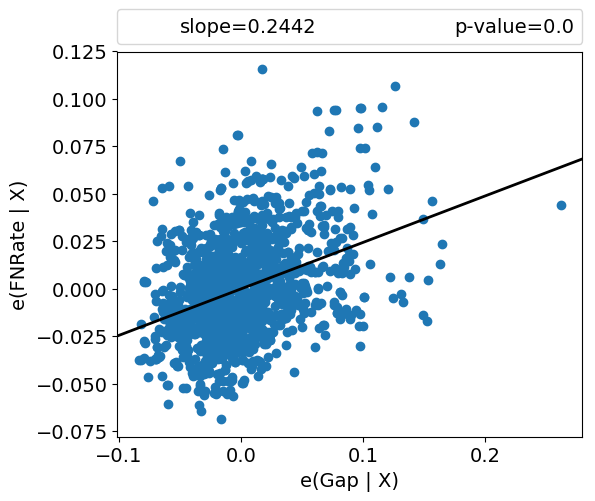
\includegraphics[width=0.25\textwidth]{Figure/NumGaps_SOP_TC_wSOP/precomputedInit/R0/fig/gap_partial_regression}} & 
			\raisebox{-.5\height}{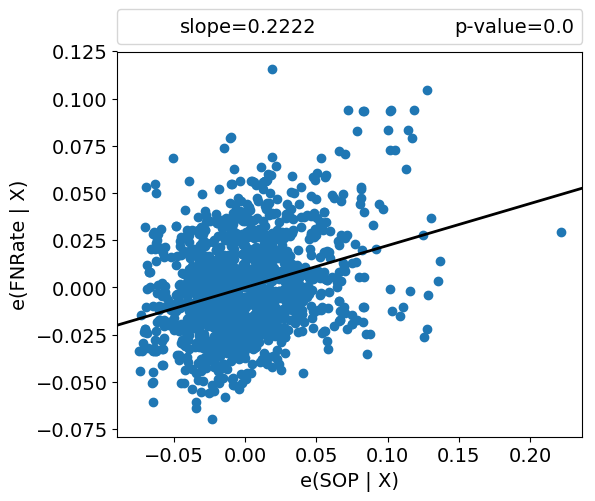
\includegraphics[width=0.25\textwidth]{Figure/NumGaps_SOP_TC_wSOP/precomputedInit/R0/fig/sop_partial_regression}} & 
			\raisebox{-.5\height}{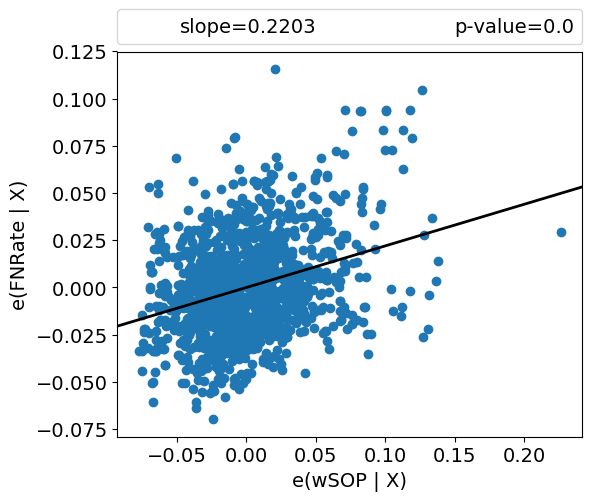
\includegraphics[width=0.25\textwidth]{Figure/NumGaps_SOP_TC_wSOP/precomputedInit/R0/fig/wsop_partial_regression}} 	
			\\\hline
			\rotatebox[origin=c]{-90}{R4} &
			\raisebox{-.5\height}{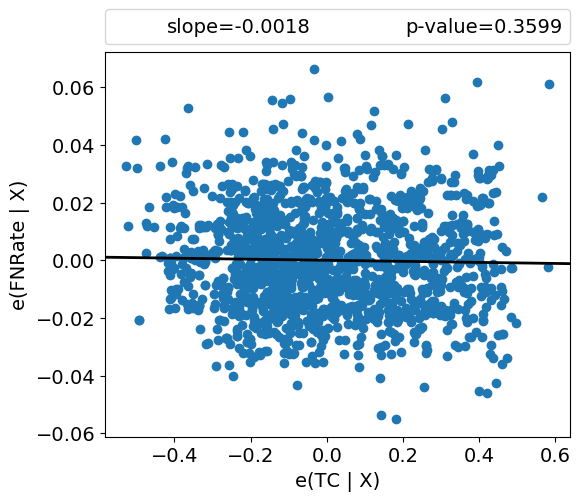
\includegraphics[width=0.25\textwidth]{Figure/NumGaps_SOP_TC_wSOP/precomputedInit/R4/fig/tc_partial_regression}} &
			\raisebox{-.5\height}{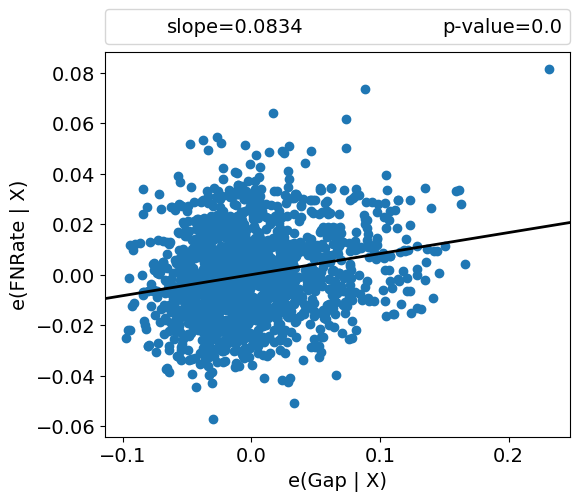
\includegraphics[width=0.25\textwidth]{Figure/NumGaps_SOP_TC_wSOP/precomputedInit/R4/fig/gap_partial_regression}} & 
			\raisebox{-.5\height}{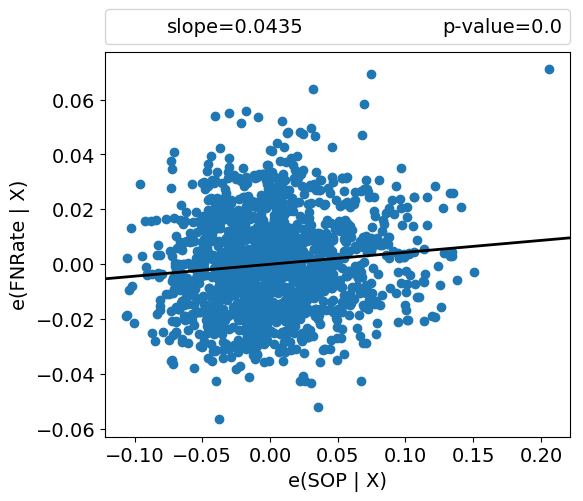
\includegraphics[width=0.25\textwidth]{Figure/NumGaps_SOP_TC_wSOP/precomputedInit/R4/fig/sop_partial_regression}} & 
			\raisebox{-.5\height}{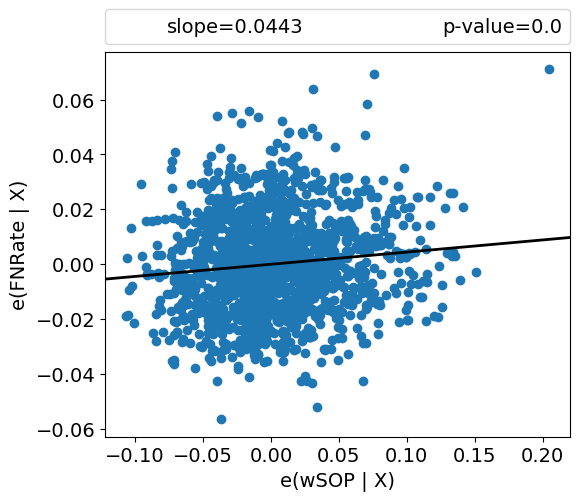
\includegraphics[width=0.25\textwidth]{Figure/NumGaps_SOP_TC_wSOP/precomputedInit/R4/fig/wsop_partial_regression}}
			\\\hline
			\rotatebox[origin=c]{-90}{R9} &
			\raisebox{-.5\height}{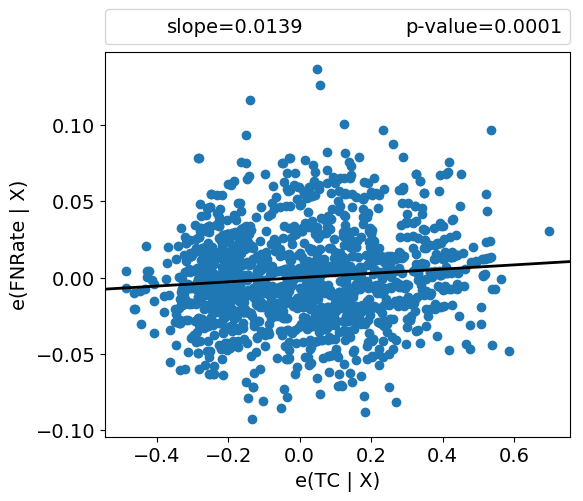
\includegraphics[width=0.25\textwidth]{Figure/NumGaps_SOP_TC_wSOP/precomputedInit/R9/fig/tc_partial_regression}} &
			\raisebox{-.5\height}{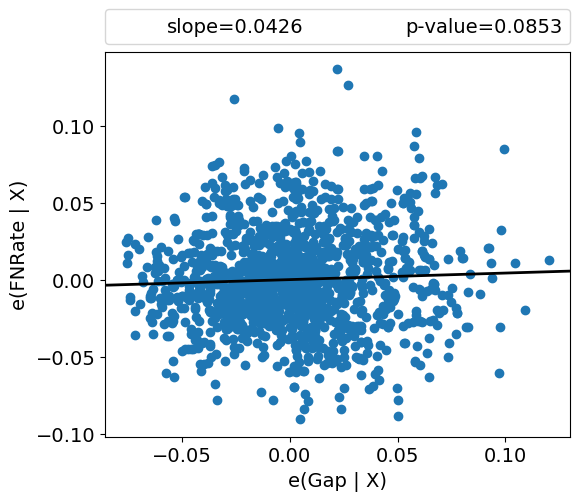
\includegraphics[width=0.25\textwidth]{Figure/NumGaps_SOP_TC_wSOP/precomputedInit/R9/fig/gap_partial_regression}} & 
			\raisebox{-.5\height}{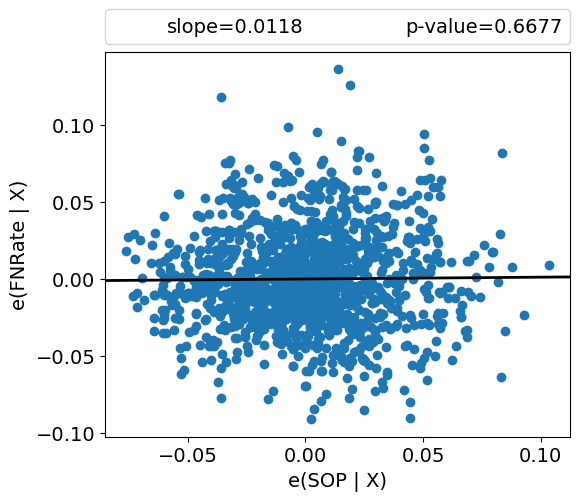
\includegraphics[width=0.25\textwidth]{Figure/NumGaps_SOP_TC_wSOP/precomputedInit/R9/fig/sop_partial_regression}} & 
			\raisebox{-.5\height}{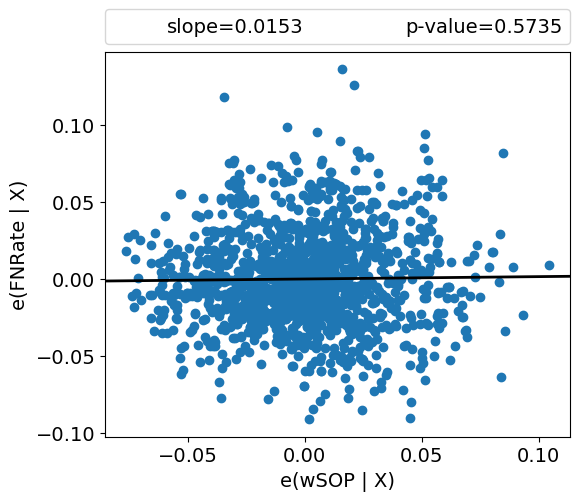
\includegraphics[width=0.25\textwidth]{Figure/NumGaps_SOP_TC_wSOP/precomputedInit/R9/fig/wsop_partial_regression}}
			\\\hline
			\rotatebox[origin=c]{-90}{R14} &
			\raisebox{-.5\height}{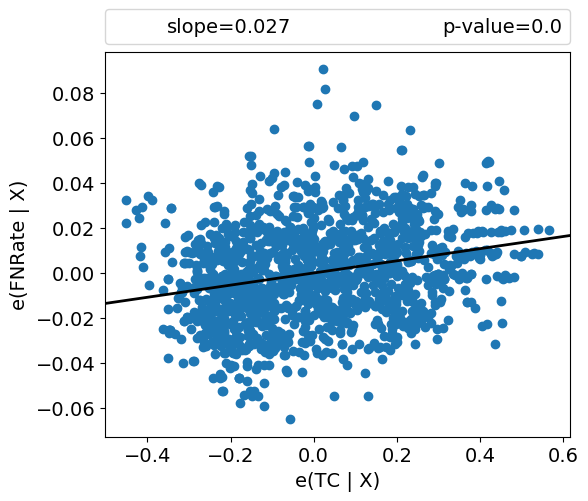
\includegraphics[width=0.25\textwidth]{Figure/NumGaps_SOP_TC_wSOP/precomputedInit/R14/fig/tc_partial_regression}} &
			\raisebox{-.5\height}{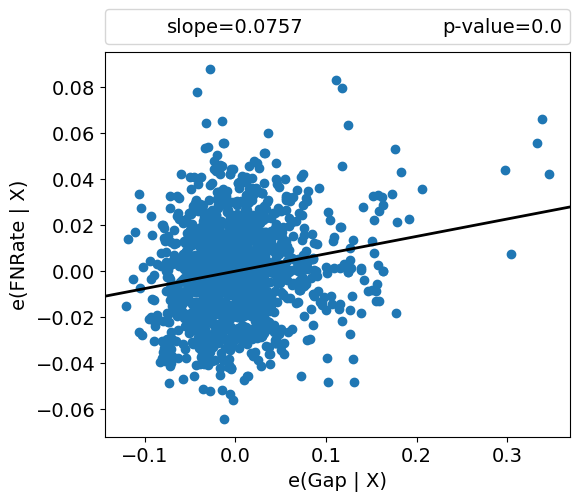
\includegraphics[width=0.25\textwidth]{Figure/NumGaps_SOP_TC_wSOP/precomputedInit/R14/fig/gap_partial_regression}} & 
			\raisebox{-.5\height}{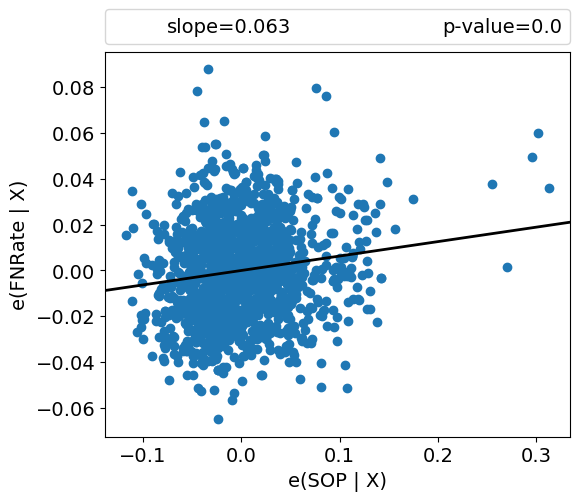
\includegraphics[width=0.25\textwidth]{Figure/NumGaps_SOP_TC_wSOP/precomputedInit/R14/fig/sop_partial_regression}} & 
			\raisebox{-.5\height}{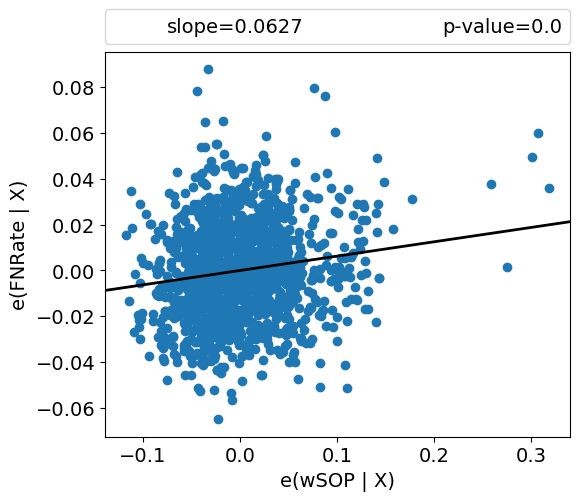
\includegraphics[width=0.25\textwidth]{Figure/NumGaps_SOP_TC_wSOP/precomputedInit/R14/fig/wsop_partial_regression}}
			\\\hline
			\rotatebox[origin=c]{-90}{R19} &
			\raisebox{-.5\height}{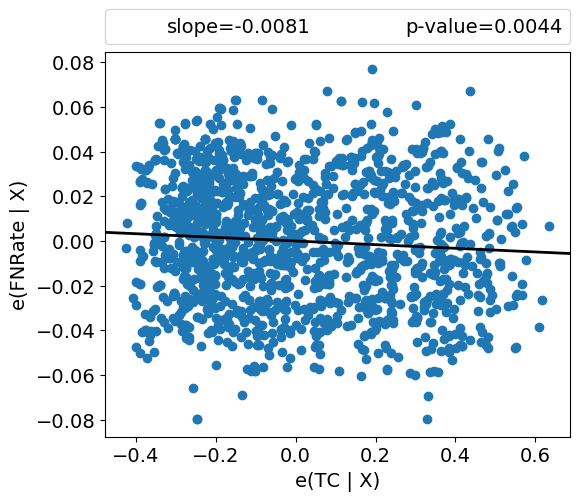
\includegraphics[width=0.25\textwidth]{Figure/NumGaps_SOP_TC_wSOP/precomputedInit/R19/fig/tc_partial_regression}} &
			\raisebox{-.5\height}{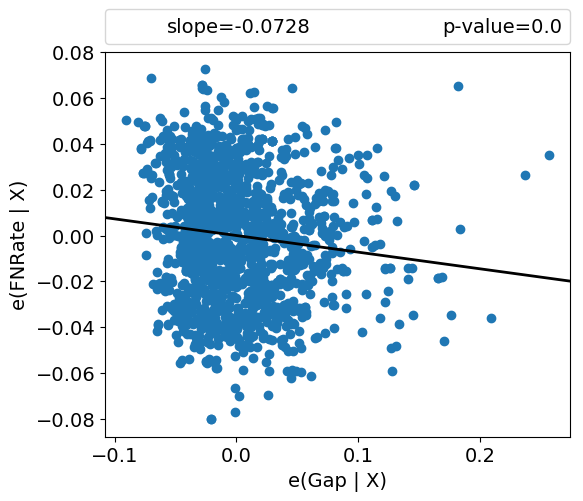
\includegraphics[width=0.25\textwidth]{Figure/NumGaps_SOP_TC_wSOP/precomputedInit/R19/fig/gap_partial_regression}} & 
			\raisebox{-.5\height}{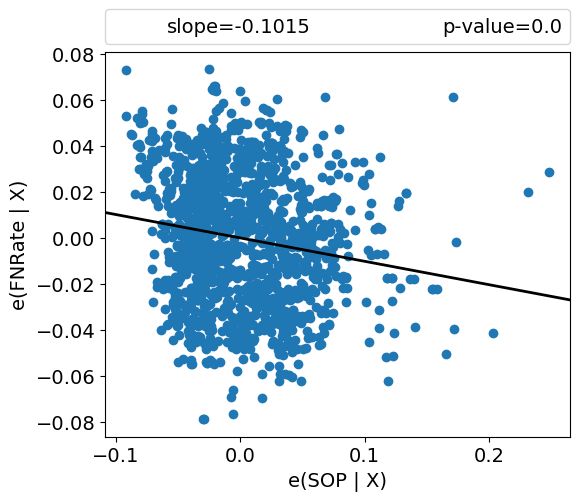
\includegraphics[width=0.25\textwidth]{Figure/NumGaps_SOP_TC_wSOP/precomputedInit/R19/fig/sop_partial_regression}} & 
			\raisebox{-.5\height}{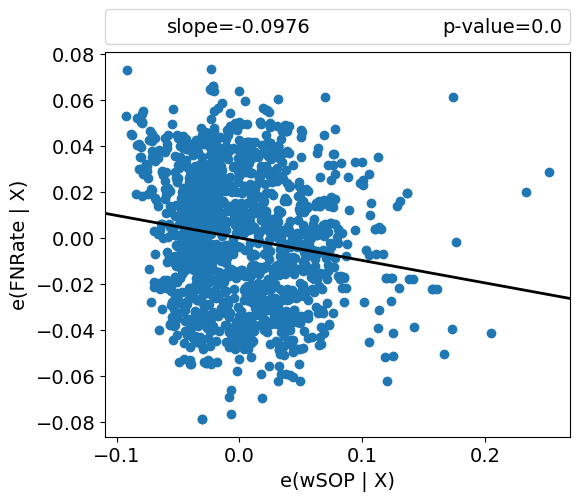
\includegraphics[width=0.25\textwidth]{Figure/NumGaps_SOP_TC_wSOP/precomputedInit/R19/fig/wsop_partial_regression}}
			\\\hline
		\end{tabular}
		\caption{\underline{100-taxon simulated dataset:} Multiple linear regression model for identifying the association among FN rate and three objective functions (TC, Gap and SOP/wSOP) fitted to five randomly selected replicates. There is one figure for each possible combination (replicate, objective function). Each partial regression plot shows the association between an objective function and FN rate while holding the remaining two objectives constant. In a plot for an objective function $ OF $, the horizontal axis, $e(OF|X)$, denotes the residuals from regressing $OF$ against the remaining objective functions and the vertical axis, $e(FNRate|X)$, denotes the residuals from regressing FN rate against all the objective functions except $ OF $.} 
		\label{fig:mul_lin_reg}
	\end{adjustwidth}
\end{figure*}

\begin{figure*}[!htbp]
	\centering
	\begin{adjustwidth}{-1cm}{-1cm}
		\begin{subfigure}{0.22\textwidth}
			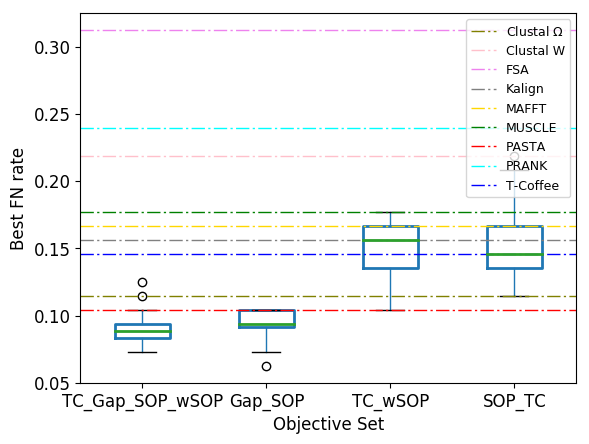
\includegraphics[width=\columnwidth]{Figure/summary/precomputedInit/R0/objset_fnrate_rank}
			\caption{R0}
			%\label{fig:con_pr09}
		\end{subfigure}	
		\begin{subfigure}{0.22\textwidth}
			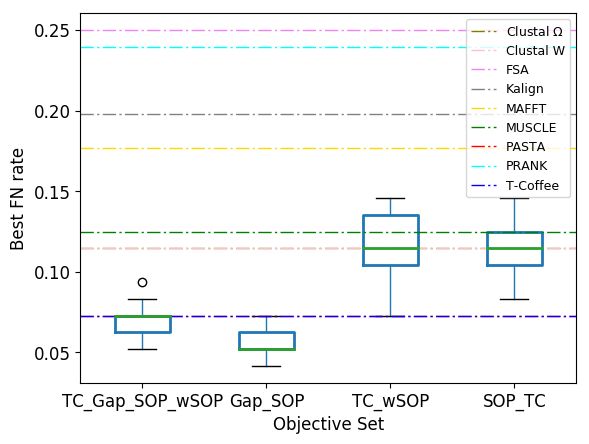
\includegraphics[width=\columnwidth]{Figure/summary/precomputedInit/R4/objset_fnrate_rank}
			\caption{R4}
			%\label{fig:con_pr09}
		\end{subfigure}
		\begin{subfigure}{0.22\textwidth}
			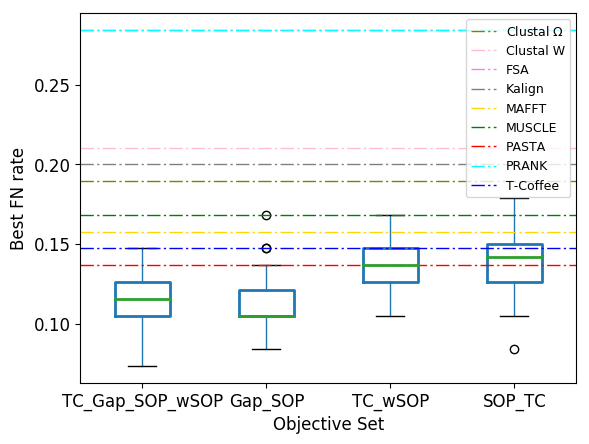
\includegraphics[width=\columnwidth]{Figure/summary/precomputedInit/R9/objset_fnrate_rank}
			\caption{R9}
			%\label{fig:con_pr09}
		\end{subfigure}
		\begin{subfigure}{0.22\textwidth}
			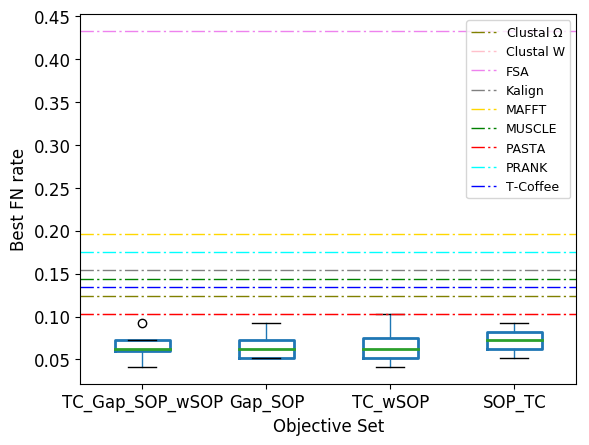
\includegraphics[width=\columnwidth]{Figure/summary/precomputedInit/R14/objset_fnrate_rank}
			\caption{R14}
			%\label{fig:con_pr09}
		\end{subfigure}
		\begin{subfigure}{0.22\textwidth}
			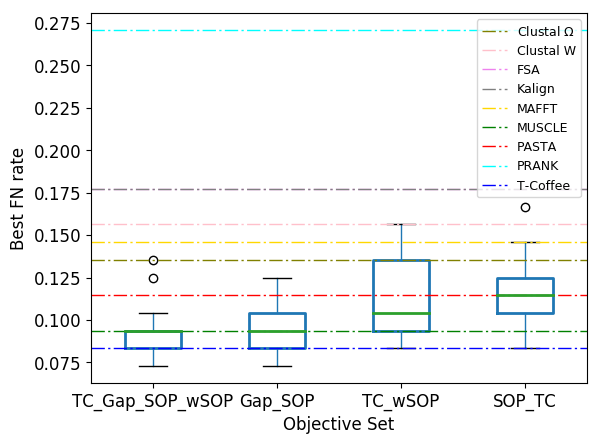
\includegraphics[width=\columnwidth]{Figure/summary/precomputedInit/R19/objset_fnrate_rank}
			\caption{R19}
			%\label{fig:con_pr09}
		\end{subfigure}
		\caption{\underline{100-taxon simulated dataset:} Comparison among objective sets based on the distribution of the collection of the best FN rates from each run. The performance of the state-of-the-art tools are shown using horizontal lines.}
		\label{fig:rank_best_fn_rate}
	\end{adjustwidth}
\end{figure*}


\begin{figure*}[!htbp]	
	\begin{adjustwidth}{-1cm}{-1cm}
		\centering
		\begin{subfigure}{0.35\textwidth}
			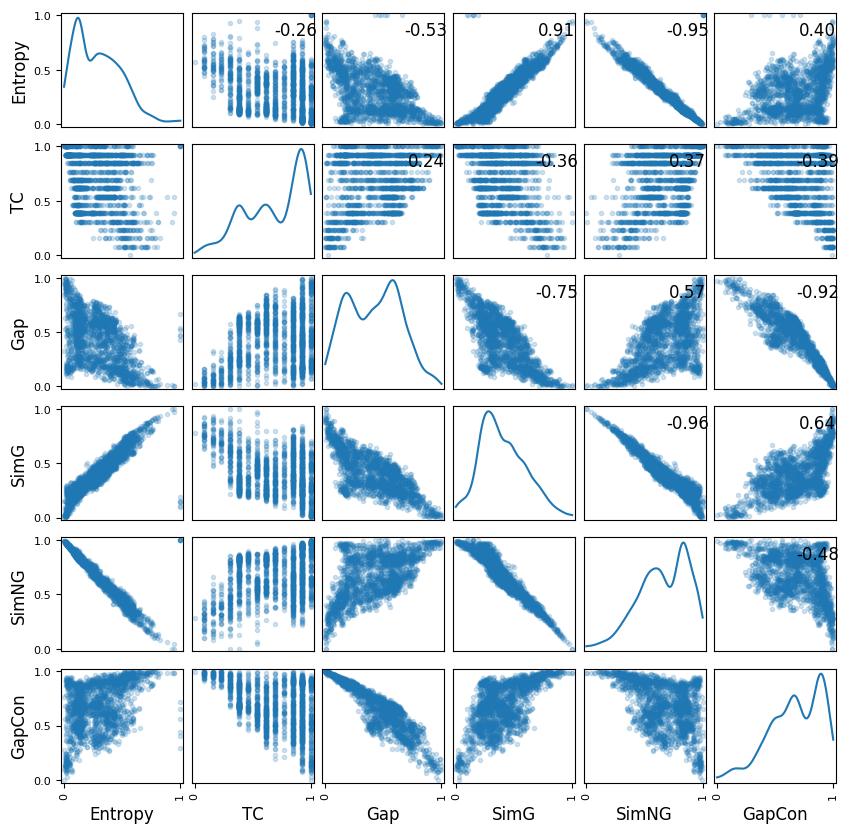
\includegraphics[width=\columnwidth]{Figure/6-obj-old/R0/fig/scatter_mattrix}
			\caption{R0}
			%\label{fig:con_pr09}
		\end{subfigure}	
		\begin{subfigure}{0.35\textwidth}
			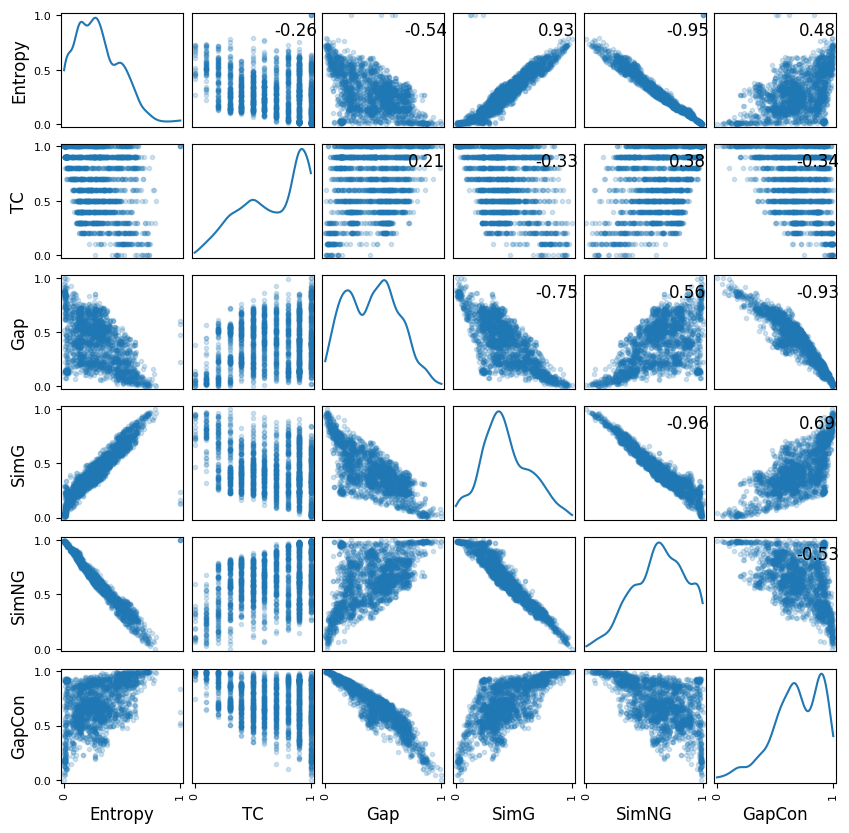
\includegraphics[width=\columnwidth]{Figure/6-obj-old/R4/fig/scatter_mattrix}
			\caption{R4}
			%\label{fig:con_pr09}
		\end{subfigure}
		\begin{subfigure}{0.35\textwidth}
			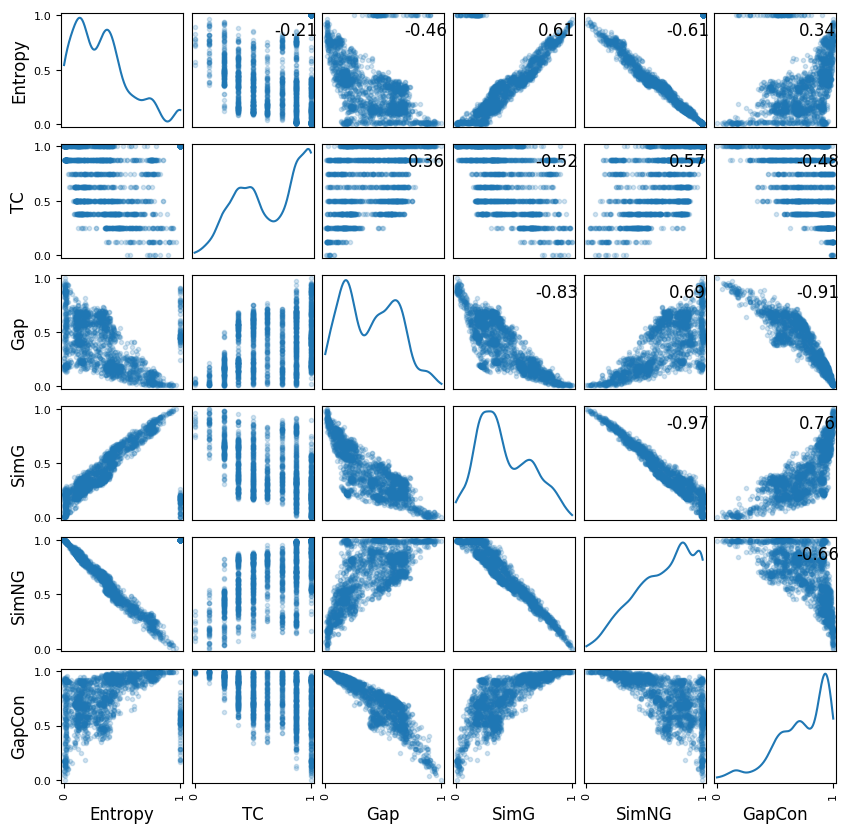
\includegraphics[width=\columnwidth]{Figure/6-obj-old/R9/fig/scatter_mattrix}
			\caption{R9}
			%\label{fig:con_pr09}
		\end{subfigure}
		\begin{subfigure}{0.35\textwidth}
			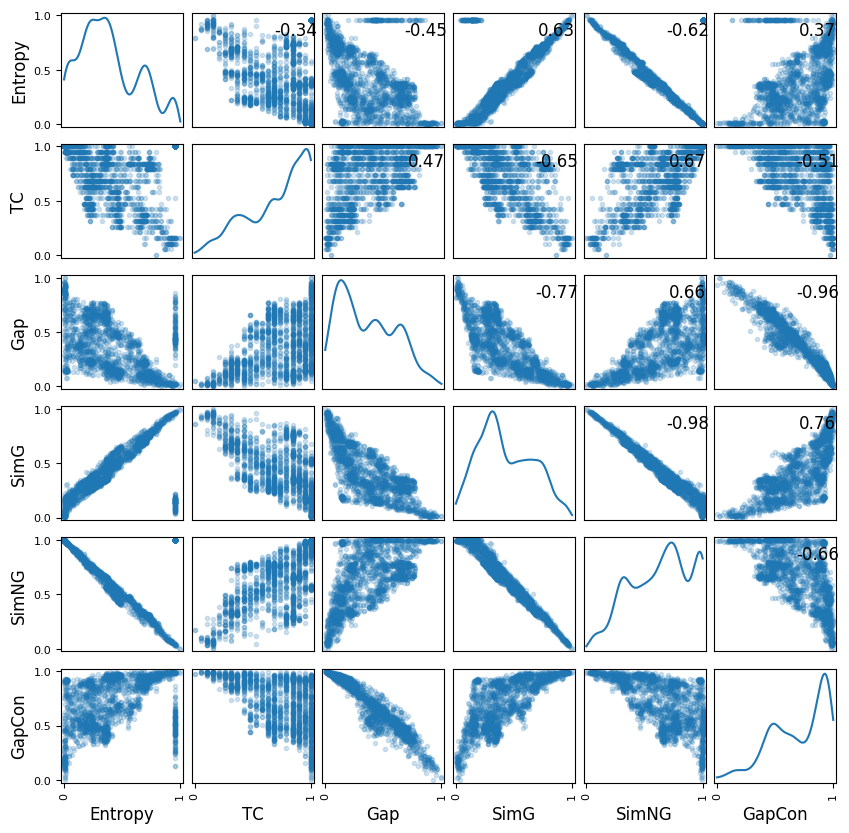
\includegraphics[width=\columnwidth]{Figure/6-obj-old/R14/fig/scatter_mattrix}
			\caption{R14}
			%\label{fig:con_pr09}
		\end{subfigure}
		\begin{subfigure}{0.35\textwidth}
			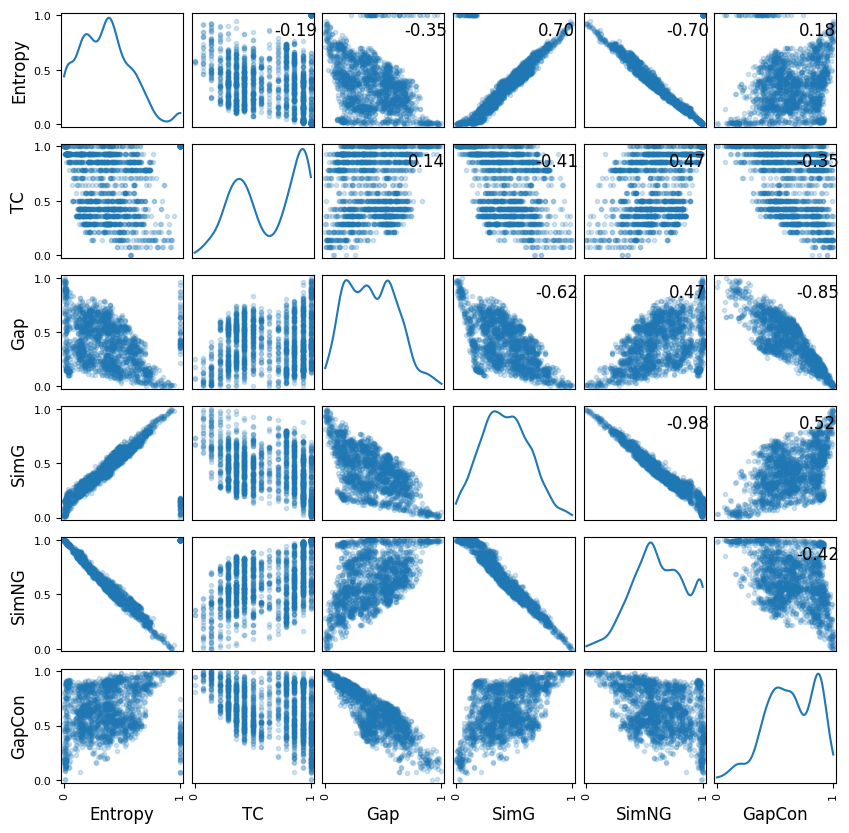
\includegraphics[width=\columnwidth]{Figure/6-obj-old/R19/fig/scatter_mattrix}
			\caption{R19}
			%\label{fig:con_pr09}
		\end{subfigure}
		\caption{\underline{100-taxon simulated dataset:} Scatter-plot matrices depicting the pairwise relationship of all objective functions on five randomly selected replicates. We turn each objective function into minimization form and then normalize using min-max technique. In each matrix, the diagonal cells show the distribution of objective values (estimated using kernel density estimation which is a non-parametric way to estimate the probability density function of a random variable) while the non-diagonal cells show the correlation between pairs of objective functions. Each upper-diagonal cell contains the value of correlation coefficient $r$ of the corresponding pair of objective functions.}
		\label{fig:new_nature_obj}
	\end{adjustwidth}
\end{figure*}
\begin{figure*}[!htbp]
	\centering
	\small
	\begin{adjustwidth}{-1cm}{-1cm}
		\begin{tabular}{l||C{0.24\textwidth}|C{0.24\textwidth}|C{0.24\textwidth}|C{0.24\textwidth} }
			& Entropy & GapCon & SimG & SimNG\\\hline\hline
			\rotatebox[origin=c]{-90}{R0} & 
			\raisebox{-.5\height}{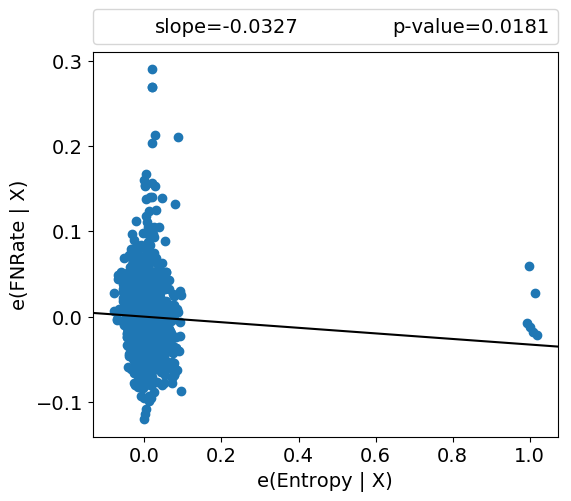
\includegraphics[width=0.25\textwidth]{Figure/6-obj-old/precomputedInit/R0/fig/Entropy_partial_regression}} &
			\raisebox{-.5\height}{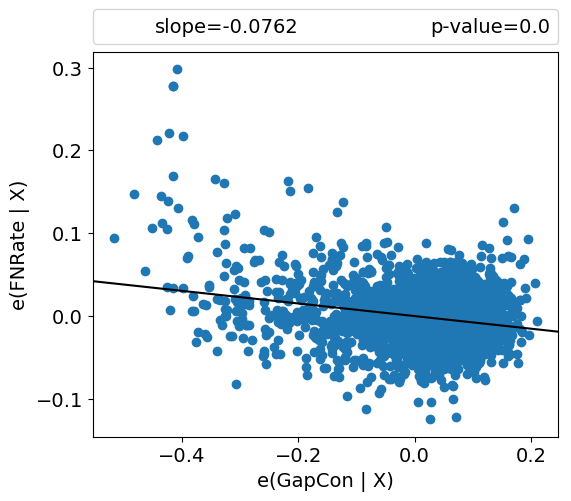
\includegraphics[width=0.25\textwidth]{Figure/6-obj-old/precomputedInit/R0/fig/GapCon_partial_regression}} & 
			\raisebox{-.5\height}{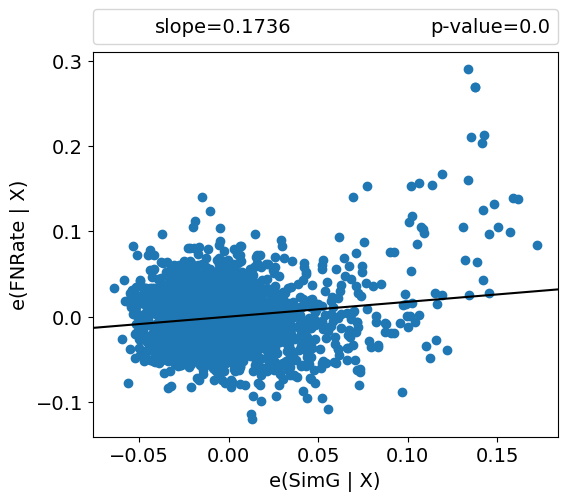
\includegraphics[width=0.25\textwidth]{Figure/6-obj-old/precomputedInit/R0/fig/SimG_partial_regression}} & 
			\raisebox{-.5\height}{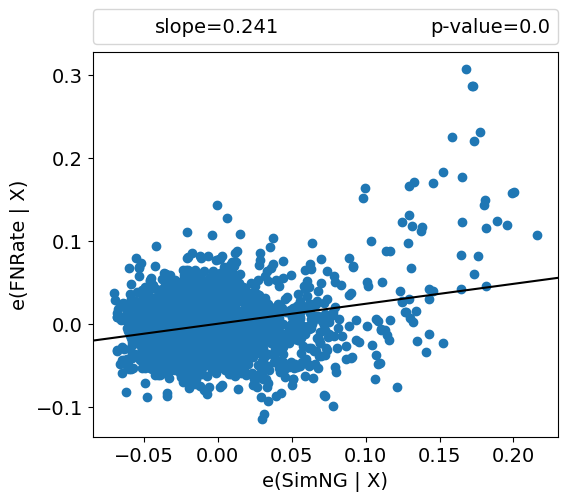
\includegraphics[width=0.25\textwidth]{Figure/6-obj-old/precomputedInit/R0/fig/SimNG_partial_regression}} 	
			\\\hline
			\rotatebox[origin=c]{-90}{R4} &
			\raisebox{-.5\height}{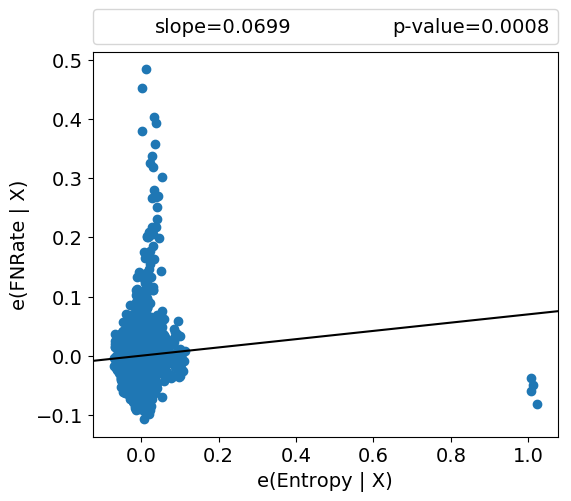
\includegraphics[width=0.25\textwidth]{Figure/6-obj-old/precomputedInit/R4/fig/Entropy_partial_regression}} &
			\raisebox{-.5\height}{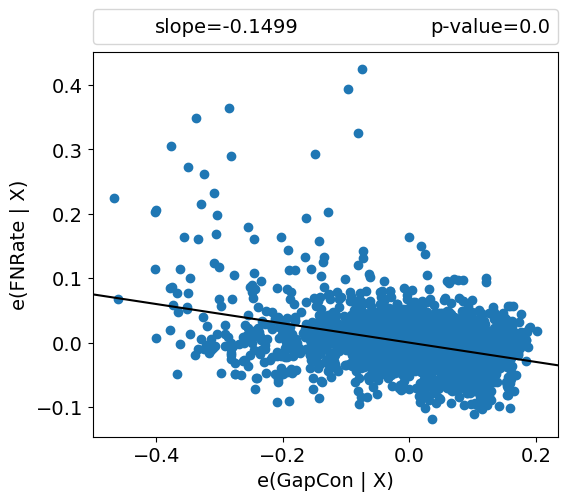
\includegraphics[width=0.25\textwidth]{Figure/6-obj-old/precomputedInit/R4/fig/GapCon_partial_regression}} & 
			\raisebox{-.5\height}{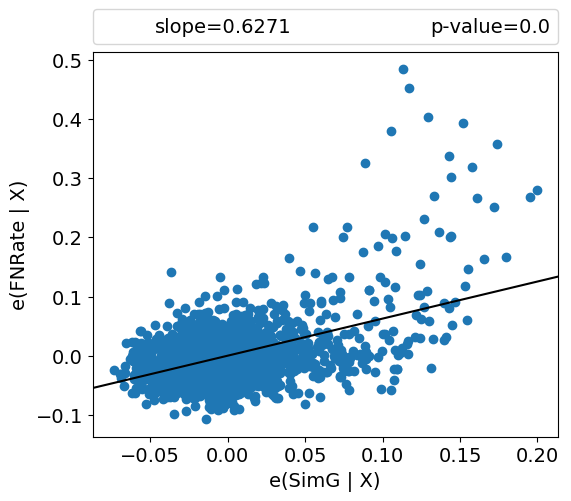
\includegraphics[width=0.25\textwidth]{Figure/6-obj-old/precomputedInit/R4/fig/SimG_partial_regression}} & 
			\raisebox{-.5\height}{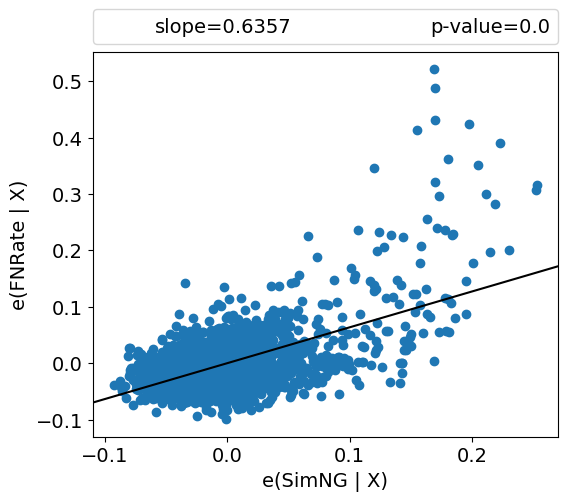
\includegraphics[width=0.25\textwidth]{Figure/6-obj-old/precomputedInit/R4/fig/SimNG_partial_regression}}
			\\\hline
			\rotatebox[origin=c]{-90}{R9} &
			\raisebox{-.5\height}{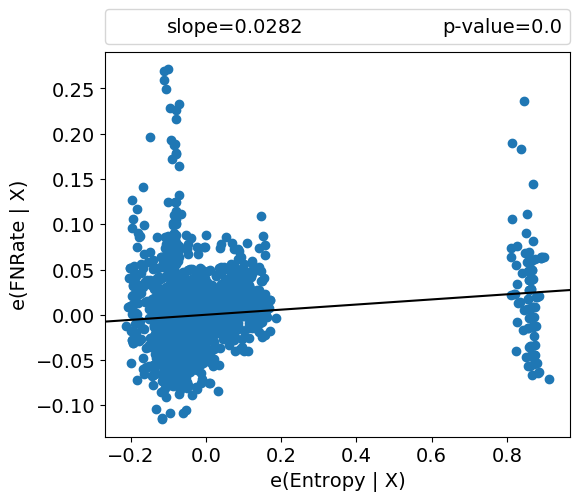
\includegraphics[width=0.25\textwidth]{Figure/6-obj-old/precomputedInit/R9/fig/Entropy_partial_regression}} &
			\raisebox{-.5\height}{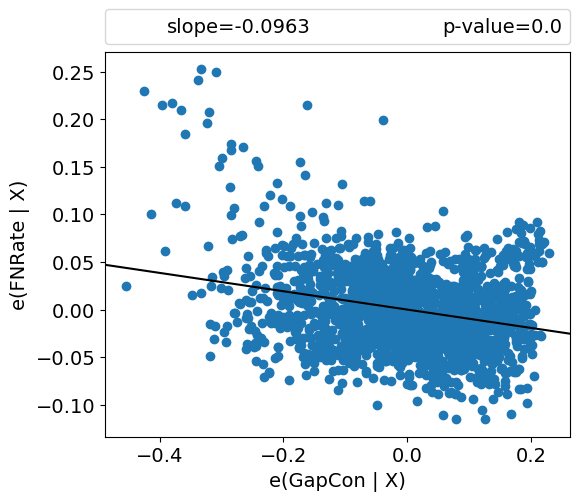
\includegraphics[width=0.25\textwidth]{Figure/6-obj-old/precomputedInit/R9/fig/GapCon_partial_regression}} & 
			\raisebox{-.5\height}{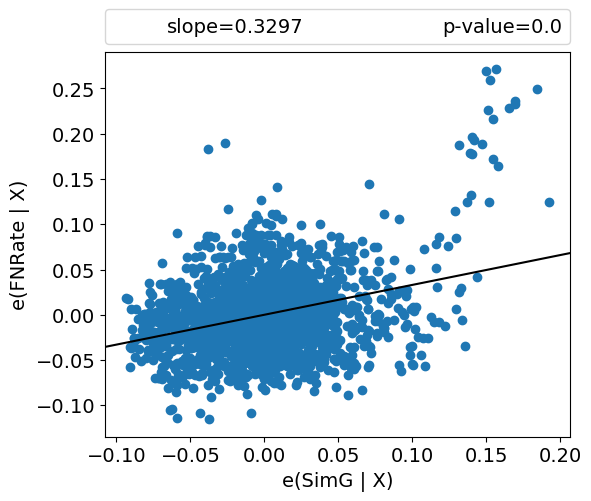
\includegraphics[width=0.25\textwidth]{Figure/6-obj-old/precomputedInit/R9/fig/SimG_partial_regression}} & 
			\raisebox{-.5\height}{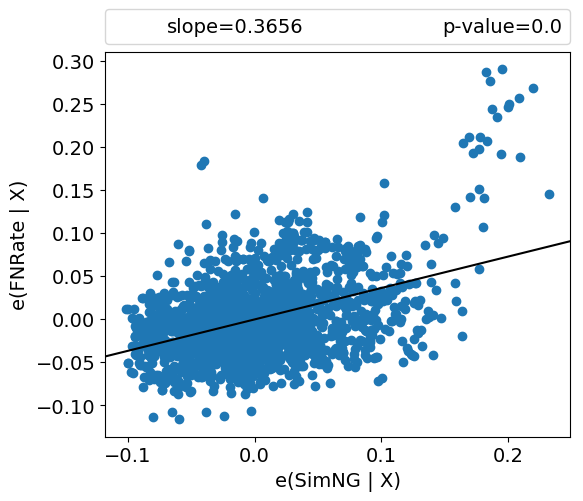
\includegraphics[width=0.25\textwidth]{Figure/6-obj-old/precomputedInit/R9/fig/SimNG_partial_regression}}
			\\\hline
			\rotatebox[origin=c]{-90}{R14} &
			\raisebox{-.5\height}{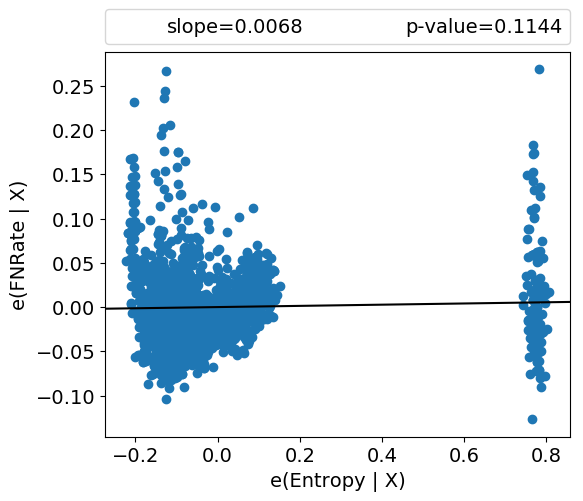
\includegraphics[width=0.25\textwidth]{Figure/6-obj-old/precomputedInit/R14/fig/Entropy_partial_regression}} &
			\raisebox{-.5\height}{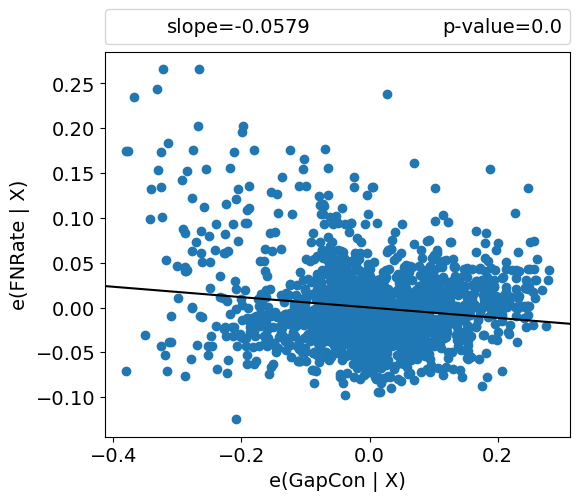
\includegraphics[width=0.25\textwidth]{Figure/6-obj-old/precomputedInit/R14/fig/GapCon_partial_regression}} & 
			\raisebox{-.5\height}{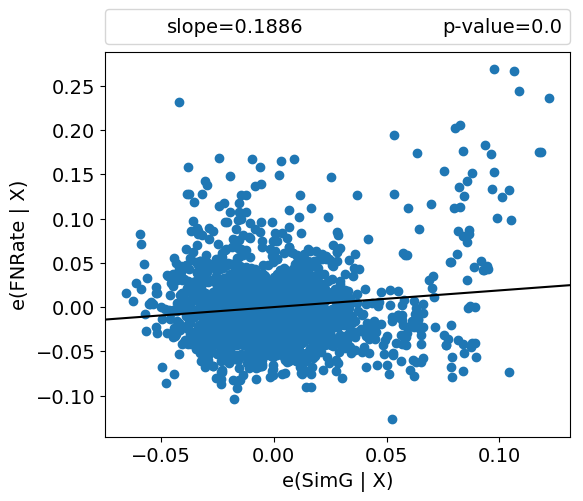
\includegraphics[width=0.25\textwidth]{Figure/6-obj-old/precomputedInit/R14/fig/SimG_partial_regression}} & 
			\raisebox{-.5\height}{\includegraphics[width=0.25\textwidth]{Figure/6-obj-old/precomputedInit/R14/fig/SimNG_partial_regression}}
			\\\hline
			\rotatebox[origin=c]{-90}{R19} &
			\raisebox{-.5\height}{\includegraphics[width=0.25\textwidth]{Figure/6-obj-old/precomputedInit/R19/fig/Entropy_partial_regression}} &
			\raisebox{-.5\height}{\includegraphics[width=0.25\textwidth]{Figure/6-obj-old/precomputedInit/R19/fig/GapCon_partial_regression}} & 
			\raisebox{-.5\height}{\includegraphics[width=0.25\textwidth]{Figure/6-obj-old/precomputedInit/R19/fig/SimG_partial_regression}} & 
			\raisebox{-.5\height}{\includegraphics[width=0.25\textwidth]{Figure/6-obj-old/precomputedInit/R19/fig/SimNG_partial_regression}}
			\\\hline
		\end{tabular}	
		\caption{\underline{100-taxon simulated dataset:} Multiple linear regression model for identifying the association among FN rate and three objective functions (SimNG, GapCon and SimG/Entropy) fitted to five randomly selected replicates. There is one figure for each possible combination (replicate, objective function). Each partial regression plot shows the association between an objective function and FN rate while holding the remaining two objectives constant.  In a plot for an objective function $ OF $, the horizontal axis, $e(OF|X)$, denotes the residuals from regressing $OF$ against the remaining objective functions and the vertical axis, $e(FNRate|X)$, denotes the residuals from regressing FN rate against all the objective functions except $ OF $.}
		\label{fig:new_mul_lin_reg}
	\end{adjustwidth}
\end{figure*}
\clearpage
\subsection{Further results on BAliBASE datasets}
Here we first discuss our findings for the five datasets under group RV12. Here According to FN rate (Figure \ref{fig:rv12_fn_rate}), the multi-objective formulations outperform all the state-of-the-art tools for BB12013 and BB12035. In case of BB12035, \{SimG, SimNG\} reconstructs all the edges correctly as opposed to 20\% FN rate attained by the trees estimated on the MSA generated by the best tool which is remarkable.
%shows remarkable improvement in FN rate \commentA{(0\% vs 20\%)}\footnote{\commentA{Here I mean, our approach achieves 0\% FN rate while the best tool achieves 20\% Fn rate}} compared to the best tool. 
For the remaining datasets (BB12001 and BB12022), the multi-objective formulations perform as good as the best tool. On all the datasets, the two objective sets generate several solutions that are equivalent or better than that of the best tool.
%the two objective sets generate several solutions that are similar to or better than the best tool on all the datasets. And the set \{SimG, SimNG\} performs better than \{Gap, SOP\} except for BB12044. 
However, as observed in previous datasets, we see contrasting results with respect to TC and SP score (Figure \ref{fig:rv12_tc},\ref{fig:rv12_sp}). Here we find only a few cases where the two objective sets can outperform the best tool. We closely analyze this issue in Figure~\ref{fig:rv12_fnrate_vs_tc} where we find that there are several solutions that achieve better FN rates in spite of their poor alignment quality (TC and SP score). For the remaining groups, our obtained results are similar. For the sake of brevity, we only illustrate the results in Figures \ref{fig:rv20_fn_rate} to \ref{fig:rv50_fnrate_vs_tc}.
%############################# RV12
\begin{figure*}[!htbp]
	\centering
	\begin{adjustwidth}{-1cm}{-1cm}
		\begin{subfigure}{0.22\textwidth}
			\includegraphics[width=\columnwidth]{Figure/summary/precomputedInit/Balibase/BB12001_fnrate_density_single_run}
			\caption{BB12001}
			%\label{fig:con_pr09}
		\end{subfigure}	
		\begin{subfigure}{0.22\textwidth}
			\includegraphics[width=\columnwidth]{Figure/summary/precomputedInit/Balibase/BB12013_fnrate_density_single_run}
			\caption{BB12013}
			%\label{fig:con_pr09}
		\end{subfigure}
		\begin{subfigure}{0.22\textwidth}
			\includegraphics[width=\columnwidth]{Figure/summary/precomputedInit/Balibase/BB12022_fnrate_density_single_run}
			\caption{BB12022}
			%\label{fig:con_pr09}
		\end{subfigure}
		\begin{subfigure}{0.22\textwidth}
			\includegraphics[width=\columnwidth]{Figure/summary/precomputedInit/Balibase/BB12035_fnrate_density_single_run}
			\caption{BB12035}
			%\label{fig:con_pr09}
		\end{subfigure}
		\begin{subfigure}{0.22\textwidth}
			\includegraphics[width=\columnwidth]{Figure/summary/precomputedInit/Balibase/BB12044_fnrate_density_single_run}
			\caption{BB12044}
			%\label{fig:con_pr09}
		\end{subfigure}
		\begin{subfigure}{0.22\textwidth}
			\includegraphics[width=\columnwidth]{Figure/summary/precomputedInit/Balibase/BB12001_objset_fnrate_rank}
			\caption{BB12001}
			%\label{fig:con_pr09}
		\end{subfigure}	
		\begin{subfigure}{0.22\textwidth}
			\includegraphics[width=\columnwidth]{Figure/summary/precomputedInit/Balibase/BB12013_objset_fnrate_rank}
			\caption{BB12013}
			%\label{fig:con_pr09}
		\end{subfigure}
		\begin{subfigure}{0.22\textwidth}
			\includegraphics[width=\columnwidth]{Figure/summary/precomputedInit/Balibase/BB12022_objset_fnrate_rank}
			\caption{BB12022}
			%\label{fig:con_pr09}
		\end{subfigure}
		\begin{subfigure}{0.22\textwidth}
			\includegraphics[width=\columnwidth]{Figure/summary/precomputedInit/Balibase/BB12035_objset_fnrate_rank}
			\caption{BB12035}
			%\label{fig:con_pr09}
		\end{subfigure}
		\begin{subfigure}{0.22\textwidth}
			\includegraphics[width=\columnwidth]{Figure/summary/precomputedInit/Balibase/BB12044_objset_fnrate_rank}
			\caption{BB12044}
			%\label{fig:con_pr09}
		\end{subfigure}
		\caption{\underline{RV12:} Top panel (part (a) - (e)) shows the FN rate of 100 solutions averaged over 20 runs. At first, we sort the FN rates of each solution set. Then we average the FN rates at each sorted position of all the sets. Bottom panel (part (f) - (j)) shows the distribution of the best FN rates collected from all runs. In each figure, the horizontal lines show the performance of the state-of-the-art tools.}
		\label{fig:rv12_fn_rate}
	\end{adjustwidth}
\end{figure*}


\begin{figure*}[!htbp]
	\centering
	\begin{adjustwidth}{-1cm}{-1cm}
		\begin{subfigure}{0.22\textwidth}
			\includegraphics[width=\columnwidth]{Figure/summary/precomputedInit/Balibase/BB12001_tc_density_single_run_2}
			\caption{BB12001}
			%\label{fig:con_pr09}
		\end{subfigure}	
		\begin{subfigure}{0.22\textwidth}
			\includegraphics[width=\columnwidth]{Figure/summary/precomputedInit/Balibase/BB12013_tc_density_single_run_2}
			\caption{BB12013}
			%\label{fig:con_pr09}
		\end{subfigure}
		\begin{subfigure}{0.22\textwidth}
			\includegraphics[width=\columnwidth]{Figure/summary/precomputedInit/Balibase/BB12022_tc_density_single_run_2}
			\caption{BB12022}
			%\label{fig:con_pr09}
		\end{subfigure}
		\begin{subfigure}{0.22\textwidth}
			\includegraphics[width=\columnwidth]{Figure/summary/precomputedInit/Balibase/BB12035_tc_density_single_run_2}
			\caption{BB12035}
			%\label{fig:con_pr09}
		\end{subfigure}
		\begin{subfigure}{0.22\textwidth}
			\includegraphics[width=\columnwidth]{Figure/summary/precomputedInit/Balibase/BB12044_tc_density_single_run_2}
			\caption{BB12044}
			%\label{fig:con_pr09}
		\end{subfigure}
		%%%%%%%%%%%%%%
		\begin{subfigure}{0.22\textwidth}
			\includegraphics[width=\columnwidth]{Figure/summary/precomputedInit/Balibase/BB12001_objset_tc_rank_2}
			\caption{BB12001}
			%\label{fig:con_pr09}
		\end{subfigure}	
		\begin{subfigure}{0.22\textwidth}
			\includegraphics[width=\columnwidth]{Figure/summary/precomputedInit/Balibase/BB12013_objset_tc_rank_2}
			\caption{BB12013}
			%\label{fig:con_pr09}
		\end{subfigure}
		\begin{subfigure}{0.22\textwidth}
			\includegraphics[width=\columnwidth]{Figure/summary/precomputedInit/Balibase/BB12022_objset_tc_rank_2}
			\caption{BB12022}
			%\label{fig:con_pr09}
		\end{subfigure}
		\begin{subfigure}{0.22\textwidth}
			\includegraphics[width=\columnwidth]{Figure/summary/precomputedInit/Balibase/BB12035_objset_tc_rank_2}
			\caption{BB12035}
			%\label{fig:con_pr09}
		\end{subfigure}
		\begin{subfigure}{0.22\textwidth}
			\includegraphics[width=\columnwidth]{Figure/summary/precomputedInit/Balibase/BB12044_objset_tc_rank_2}
			\caption{BB12044}
			%\label{fig:con_pr09}
		\end{subfigure}
		\caption{\underline{RV12:} Top panel (part (a) - (e)) shows the TC score of 100 solutions averaged over 20 runs. At first, we sort the TC scores of each solution set. Then we average the TC scores at each sorted position of all the sets. Bottom panel (part (f) - (j)) shows the distribution of the best TC scores collected from all runs. In each figure, the horizontal lines show the performance of the state-of-the-art tools.}
		\label{fig:rv12_tc}
	\end{adjustwidth}
\end{figure*}


\begin{figure*}[!htbp]
	\centering
	\begin{adjustwidth}{-1cm}{-1cm}
		\begin{subfigure}{0.22\textwidth}
			\includegraphics[width=\columnwidth]{Figure/summary/precomputedInit/Balibase/BB12001_pairs_density_single_run_2}
			\caption{BB12001}
			%\label{fig:con_pr09}
		\end{subfigure}	
		\begin{subfigure}{0.22\textwidth}
			\includegraphics[width=\columnwidth]{Figure/summary/precomputedInit/Balibase/BB12013_pairs_density_single_run_2}
			\caption{BB12013}
			%\label{fig:con_pr09}
		\end{subfigure}
		\begin{subfigure}{0.22\textwidth}
			\includegraphics[width=\columnwidth]{Figure/summary/precomputedInit/Balibase/BB12022_pairs_density_single_run_2}
			\caption{BB12022}
			%\label{fig:con_pr09}
		\end{subfigure}
		\begin{subfigure}{0.22\textwidth}
			\includegraphics[width=\columnwidth]{Figure/summary/precomputedInit/Balibase/BB12035_pairs_density_single_run_2}
			\caption{BB12035}
			%\label{fig:con_pr09}
		\end{subfigure}
		\begin{subfigure}{0.22\textwidth}
			\includegraphics[width=\columnwidth]{Figure/summary/precomputedInit/Balibase/BB12044_pairs_density_single_run_2}
			\caption{BB12044}
			%\label{fig:con_pr09}
		\end{subfigure}
		\begin{subfigure}{0.22\textwidth}
			\includegraphics[width=\columnwidth]{Figure/summary/precomputedInit/Balibase/BB12001_objset_pairs_rank_2}
			\caption{BB12001}
			%\label{fig:con_pr09}
		\end{subfigure}	
		\begin{subfigure}{0.22\textwidth}
			\includegraphics[width=\columnwidth]{Figure/summary/precomputedInit/Balibase/BB12013_objset_pairs_rank_2}
			\caption{BB12013}
			%\label{fig:con_pr09}
		\end{subfigure}
		\begin{subfigure}{0.22\textwidth}
			\includegraphics[width=\columnwidth]{Figure/summary/precomputedInit/Balibase/BB12022_objset_pairs_rank_2}
			\caption{BB12022}
			%\label{fig:con_pr09}
		\end{subfigure}
		\begin{subfigure}{0.22\textwidth}
			\includegraphics[width=\columnwidth]{Figure/summary/precomputedInit/Balibase/BB12035_objset_pairs_rank_2}
			\caption{BB12035}
			%\label{fig:con_pr09}
		\end{subfigure}
		\begin{subfigure}{0.22\textwidth}
			\includegraphics[width=\columnwidth]{Figure/summary/precomputedInit/Balibase/BB12044_objset_pairs_rank_2}
			\caption{BB12044}
			%\label{fig:con_pr09}
		\end{subfigure}
		\caption{\underline{RV12:} Top panel (part (a) - (e)) shows the SP score of 100 solutions averaged over 20 runs. At first, we sort the SP scores of each solution set. Then we average the SP scores at each sorted position of all the sets. Bottom panel (part (f) - (j)) shows the distribution of the best SP scores collected from all runs. In each figure, the horizontal lines show the performance of the state-of-the-art tools.}
		\label{fig:rv12_sp}
	\end{adjustwidth}
\end{figure*}


\begin{figure*}[!htbp]
	\centering
	\begin{adjustwidth}{-1cm}{-1cm}
		\begin{subfigure}{0.22\textwidth}
			\includegraphics[width=\columnwidth]{Figure/summary/precomputedInit/Balibase/BB12001_fnrate_vs_tc_2}
			\caption{BB12001}
			%\label{fig:con_pr09}
		\end{subfigure}	
		\begin{subfigure}{0.22\textwidth}
			\includegraphics[width=\columnwidth]{Figure/summary/precomputedInit/Balibase/BB12013_fnrate_vs_tc_2}
			\caption{BB12013}
			%\label{fig:con_pr09}
		\end{subfigure}
		\begin{subfigure}{0.22\textwidth}
			\includegraphics[width=\columnwidth]{Figure/summary/precomputedInit/Balibase/BB12022_fnrate_vs_tc_2}
			\caption{BB12022}
			%\label{fig:con_pr09}
		\end{subfigure}
		\begin{subfigure}{0.22\textwidth}
			\includegraphics[width=\columnwidth]{Figure/summary/precomputedInit/Balibase/BB12035_fnrate_vs_tc_2}
			\caption{BB12035}
			%\label{fig:con_pr09}
		\end{subfigure}	
		\begin{subfigure}{0.22\textwidth}
			\includegraphics[width=\columnwidth]{Figure/summary/precomputedInit/Balibase/BB12044_fnrate_vs_tc_2}
			\caption{BB12044}
			%\label{fig:con_pr09}
		\end{subfigure}
		%%%%%%%%%
		\begin{subfigure}{0.22\textwidth}
			\includegraphics[width=\columnwidth]{Figure/summary/precomputedInit/Balibase/BB12001_fnrate_vs_sp_2}
			\caption{BB12001}
			%\label{fig:con_pr09}
		\end{subfigure}	
		\begin{subfigure}{0.22\textwidth}
			\includegraphics[width=\columnwidth]{Figure/summary/precomputedInit/Balibase/BB12013_fnrate_vs_sp_2}
			\caption{BB12013}
			%\label{fig:con_pr09}
		\end{subfigure}
		\begin{subfigure}{0.22\textwidth}
			\includegraphics[width=\columnwidth]{Figure/summary/precomputedInit/Balibase/BB12022_fnrate_vs_sp_2}
			\caption{BB12022}
			%\label{fig:con_pr09}
		\end{subfigure}
		\begin{subfigure}{0.22\textwidth}
			\includegraphics[width=\columnwidth]{Figure/summary/precomputedInit/Balibase/BB12035_fnrate_vs_sp_2}
			\caption{BB12035}
			%\label{fig:con_pr09}
		\end{subfigure}	
		\begin{subfigure}{0.22\textwidth}
			\includegraphics[width=\columnwidth]{Figure/summary/precomputedInit/Balibase/BB12044_fnrate_vs_sp_2}
			\caption{BB12044}
			%\label{fig:con_pr09}
		\end{subfigure}
		\caption{\underline{RV12}: Top panel (part (a) - (e)) shows the relationship between FN rate and TC score for different alignments. And bottom panel (part (f) - (j)) shows the relationship between FN rate and SP score. The horizontal lines mark the FN rates achieved by the state-of-the-art tools.}
		\label{fig:rv12_fnrate_vs_tc}
	\end{adjustwidth}
\end{figure*}
%############################# RV20
\begin{figure*}[!htbp]
	\centering
	\begin{adjustwidth}{-1cm}{-1cm}
		\begin{subfigure}{0.22\textwidth}
			\includegraphics[width=\columnwidth]{Figure/summary/precomputedInit/Balibase/BB20001_fnrate_density_single_run}
			\caption{BB20001}
			%\label{fig:con_pr09}
		\end{subfigure}	
		\begin{subfigure}{0.22\textwidth}
			\includegraphics[width=\columnwidth]{Figure/summary/precomputedInit/Balibase/BB20010_fnrate_density_single_run}
			\caption{BB20010}
			%\label{fig:con_pr09}
		\end{subfigure}
		\begin{subfigure}{0.22\textwidth}
			\includegraphics[width=\columnwidth]{Figure/summary/precomputedInit/Balibase/BB20022_fnrate_density_single_run}
			\caption{BB20022}
			%\label{fig:con_pr09}
		\end{subfigure}
		\begin{subfigure}{0.22\textwidth}
			\includegraphics[width=\columnwidth]{Figure/summary/precomputedInit/Balibase/BB20033_fnrate_density_single_run}
			\caption{BB20033}
			%\label{fig:con_pr09}
		\end{subfigure}
		\begin{subfigure}{0.22\textwidth}
			\includegraphics[width=\columnwidth]{Figure/summary/precomputedInit/Balibase/BB20041_fnrate_density_single_run}
			\caption{BB20041}
			%\label{fig:con_pr09}
		\end{subfigure}
		\begin{subfigure}{0.22\textwidth}
			\includegraphics[width=\columnwidth]{Figure/summary/precomputedInit/Balibase/BB20001_objset_fnrate_rank}
			\caption{BB20001}
			%\label{fig:con_pr09}
		\end{subfigure}	
		\begin{subfigure}{0.22\textwidth}
			\includegraphics[width=\columnwidth]{Figure/summary/precomputedInit/Balibase/BB20010_objset_fnrate_rank}
			\caption{BB20010}
			%\label{fig:con_pr09}
		\end{subfigure}
		\begin{subfigure}{0.22\textwidth}
			\includegraphics[width=\columnwidth]{Figure/summary/precomputedInit/Balibase/BB20022_objset_fnrate_rank}
			\caption{BB20022}
			%\label{fig:con_pr09}
		\end{subfigure}
		\begin{subfigure}{0.22\textwidth}
			\includegraphics[width=\columnwidth]{Figure/summary/precomputedInit/Balibase/BB20033_objset_fnrate_rank}
			\caption{BB20033}
			%\label{fig:con_pr09}
		\end{subfigure}
		\begin{subfigure}{0.22\textwidth}
			\includegraphics[width=\columnwidth]{Figure/summary/precomputedInit/Balibase/BB20041_objset_fnrate_rank}
			\caption{BB20041}
			%\label{fig:con_pr09}
		\end{subfigure}
		\caption{\underline{RV20:} Top panel (part (a) - (d)) shows the FN rate of 100 final solutions averaged over 20 runs. At first, we sort the FN rates of each solution set. Then we average the FN rates at each sorted position of all the sets. Bottom panel (part (e) - (h)) shows the distribution of the best FN rates collected from all runs. In each figure, the horizontal lines show the performance of the state-of-the-art tools.}
		\label{fig:rv20_fn_rate}
	\end{adjustwidth}
\end{figure*}


\begin{figure*}[!htbp]
	\centering
	\begin{adjustwidth}{-1cm}{-1cm}
		\begin{subfigure}{0.22\textwidth}
			\includegraphics[width=\columnwidth]{Figure/summary/precomputedInit/Balibase/BB20001_tc_density_single_run_2}
			\caption{BB20001}
			%\label{fig:con_pr09}
		\end{subfigure}	
		\begin{subfigure}{0.22\textwidth}
			\includegraphics[width=\columnwidth]{Figure/summary/precomputedInit/Balibase/BB20010_tc_density_single_run_2}
			\caption{BB20010}
			%\label{fig:con_pr09}
		\end{subfigure}
		\begin{subfigure}{0.22\textwidth}
			\includegraphics[width=\columnwidth]{Figure/summary/precomputedInit/Balibase/BB20022_tc_density_single_run_2}
			\caption{BB20022}
			%\label{fig:con_pr09}
		\end{subfigure}
		\begin{subfigure}{0.22\textwidth}
			\includegraphics[width=\columnwidth]{Figure/summary/precomputedInit/Balibase/BB20033_tc_density_single_run_2}
			\caption{BB20033}
			%\label{fig:con_pr09}
		\end{subfigure}
		\begin{subfigure}{0.22\textwidth}
			\includegraphics[width=\columnwidth]{Figure/summary/precomputedInit/Balibase/BB20041_tc_density_single_run_2}
			\caption{BB20041}
			%\label{fig:con_pr09}
		\end{subfigure}
		\begin{subfigure}{0.22\textwidth}
			\includegraphics[width=\columnwidth]{Figure/summary/precomputedInit/Balibase/BB20001_objset_tc_rank_2}
			\caption{BB20001}
			%\label{fig:con_pr09}
		\end{subfigure}	
		\begin{subfigure}{0.22\textwidth}
			\includegraphics[width=\columnwidth]{Figure/summary/precomputedInit/Balibase/BB20010_objset_tc_rank_2}
			\caption{BB20010}
			%\label{fig:con_pr09}
		\end{subfigure}
		\begin{subfigure}{0.22\textwidth}
			\includegraphics[width=\columnwidth]{Figure/summary/precomputedInit/Balibase/BB20022_objset_tc_rank_2}
			\caption{BB20022}
			%\label{fig:con_pr09}
		\end{subfigure}
		\begin{subfigure}{0.22\textwidth}
			\includegraphics[width=\columnwidth]{Figure/summary/precomputedInit/Balibase/BB20033_objset_tc_rank_2}
			\caption{BB20033}
			%\label{fig:con_pr09}
		\end{subfigure}
		\begin{subfigure}{0.22\textwidth}
			\includegraphics[width=\columnwidth]{Figure/summary/precomputedInit/Balibase/BB20041_objset_tc_rank_2}
			\caption{BB20041}
			%\label{fig:con_pr09}
		\end{subfigure}
		\caption{\underline{RV20:} Top panel (part (a) - (e)) shows the TC score of 100 final solutions averaged over 20 runs. At first, we sort the TC scores of each solution set. Then we average the TC scores at each sorted position of all the sets. Bottom panel (part (f) - (j)) shows the distribution of the best TC scores collected from all runs. In each figure, the horizontal lines show the performance of the state-of-the-art tools.}
		\label{fig:rv20_tc}
	\end{adjustwidth}
\end{figure*}

\begin{figure*}[!htbp]
	\centering
	\begin{adjustwidth}{-1cm}{-1cm}
		\begin{subfigure}{0.22\textwidth}
			\includegraphics[width=\columnwidth]{Figure/summary/precomputedInit/Balibase/BB20001_pairs_density_single_run_2}
			\caption{BB20001}
			%\label{fig:con_pr09}
		\end{subfigure}	
		\begin{subfigure}{0.22\textwidth}
			\includegraphics[width=\columnwidth]{Figure/summary/precomputedInit/Balibase/BB20010_pairs_density_single_run_2}
			\caption{BB20010}
			%\label{fig:con_pr09}
		\end{subfigure}
		\begin{subfigure}{0.22\textwidth}
			\includegraphics[width=\columnwidth]{Figure/summary/precomputedInit/Balibase/BB20022_pairs_density_single_run_2}
			\caption{BB20022}
			%\label{fig:con_pr09}
		\end{subfigure}
		\begin{subfigure}{0.22\textwidth}
			\includegraphics[width=\columnwidth]{Figure/summary/precomputedInit/Balibase/BB20033_pairs_density_single_run_2}
			\caption{BB20033}
			%\label{fig:con_pr09}
		\end{subfigure}
		\begin{subfigure}{0.22\textwidth}
			\includegraphics[width=\columnwidth]{Figure/summary/precomputedInit/Balibase/BB20041_pairs_density_single_run_2}
			\caption{BB20041}
			%\label{fig:con_pr09}
		\end{subfigure}
		\begin{subfigure}{0.22\textwidth}
			\includegraphics[width=\columnwidth]{Figure/summary/precomputedInit/Balibase/BB20001_objset_pairs_rank_2}
			\caption{BB20001}
			%\label{fig:con_pr09}
		\end{subfigure}	
		\begin{subfigure}{0.22\textwidth}
			\includegraphics[width=\columnwidth]{Figure/summary/precomputedInit/Balibase/BB20010_objset_pairs_rank_2}
			\caption{BB20010}
			%\label{fig:con_pr09}
		\end{subfigure}
		\begin{subfigure}{0.22\textwidth}
			\includegraphics[width=\columnwidth]{Figure/summary/precomputedInit/Balibase/BB20022_objset_pairs_rank_2}
			\caption{BB20022}
			%\label{fig:con_pr09}
		\end{subfigure}
		\begin{subfigure}{0.22\textwidth}
			\includegraphics[width=\columnwidth]{Figure/summary/precomputedInit/Balibase/BB20033_objset_pairs_rank_2}
			\caption{BB20033}
			%\label{fig:con_pr09}
		\end{subfigure}
		\begin{subfigure}{0.22\textwidth}
			\includegraphics[width=\columnwidth]{Figure/summary/precomputedInit/Balibase/BB20041_objset_pairs_rank_2}
			\caption{BB20041}
			%\label{fig:con_pr09}
		\end{subfigure}
		\caption{\underline{RV20:} Top panel (part (a) - (e)) shows the SP score of 100 final solutions averaged over 20 runs. At first, we sort the SP scores of each solution set. Then we average the SP scores at each sorted position of all the sets. Bottom panel (part (f) - (j)) shows the distribution of the best SP scores collected from all runs. In each figure, the horizontal lines show the performance of the state-of-the-art tools.}
		\label{fig:rv20_sp}
	\end{adjustwidth}
\end{figure*}


\begin{figure*}[!htbp]
	\centering
	\begin{adjustwidth}{-1cm}{-1cm}
		\begin{subfigure}{0.22\textwidth}
			\includegraphics[width=\columnwidth]{Figure/summary/precomputedInit/Balibase/BB20001_fnrate_vs_tc_2}
			\caption{BB20001}
			%\label{fig:con_pr09}
		\end{subfigure}	
		\begin{subfigure}{0.22\textwidth}
			\includegraphics[width=\columnwidth]{Figure/summary/precomputedInit/Balibase/BB20010_fnrate_vs_tc_2}
			\caption{BB20010}
			%\label{fig:con_pr09}
		\end{subfigure}
		\begin{subfigure}{0.22\textwidth}
			\includegraphics[width=\columnwidth]{Figure/summary/precomputedInit/Balibase/BB20022_fnrate_vs_tc_2}
			\caption{BB20022}
			%\label{fig:con_pr09}
		\end{subfigure}
		\begin{subfigure}{0.22\textwidth}
			\includegraphics[width=\columnwidth]{Figure/summary/precomputedInit/Balibase/BB20033_fnrate_vs_tc_2}
			\caption{BB20033}
			%\label{fig:con_pr09}
		\end{subfigure}	
		\begin{subfigure}{0.22\textwidth}
			\includegraphics[width=\columnwidth]{Figure/summary/precomputedInit/Balibase/BB20041_fnrate_vs_tc_2}
			\caption{BB20041}
			%\label{fig:con_pr09}
		\end{subfigure}
		%%%%%%%%%%
		\begin{subfigure}{0.22\textwidth}
			\includegraphics[width=\columnwidth]{Figure/summary/precomputedInit/Balibase/BB20001_fnrate_vs_sp_2}
			\caption{BB20001}
			%\label{fig:con_pr09}
		\end{subfigure}	
		\begin{subfigure}{0.22\textwidth}
			\includegraphics[width=\columnwidth]{Figure/summary/precomputedInit/Balibase/BB20010_fnrate_vs_sp_2}
			\caption{BB20010}
			%\label{fig:con_pr09}
		\end{subfigure}
		\begin{subfigure}{0.22\textwidth}
			\includegraphics[width=\columnwidth]{Figure/summary/precomputedInit/Balibase/BB20022_fnrate_vs_sp_2}
			\caption{BB20022}
			%\label{fig:con_pr09}
		\end{subfigure}
		\begin{subfigure}{0.22\textwidth}
			\includegraphics[width=\columnwidth]{Figure/summary/precomputedInit/Balibase/BB20033_fnrate_vs_sp_2}
			\caption{BB20033}
			%\label{fig:con_pr09}
		\end{subfigure}	
		\begin{subfigure}{0.22\textwidth}
			\includegraphics[width=\columnwidth]{Figure/summary/precomputedInit/Balibase/BB20041_fnrate_vs_sp_2}
			\caption{BB20041}
			%\label{fig:con_pr09}
		\end{subfigure}
		\caption{\underline{RV20:} Top panel (part (a) - (e)) shows the relationship between FN rate and TC score for different alignments. And bottom panel (part (f) - (j)) shows the relationship between FN rate and SP score. The horizontal lines mark the FN rates achieved by the state-of-the-art tools.}
		\label{fig:rv20_fnrate_vs_tc}
	\end{adjustwidth}
\end{figure*}
%############################# RV30
\begin{figure*}[!htbp]
	
	\begin{adjustwidth}{-1cm}{-1cm}
		\centering
		\begin{subfigure}{0.22\textwidth}
			\includegraphics[width=\columnwidth]{Figure/summary/precomputedInit/Balibase/BB30002_fnrate_density_single_run}
			\caption{BB30002}
			%\label{fig:con_pr09}
		\end{subfigure}	
		\begin{subfigure}{0.22\textwidth}
			\includegraphics[width=\columnwidth]{Figure/summary/precomputedInit/Balibase/BB30008_fnrate_density_single_run}
			\caption{BB30008}
			%\label{fig:con_pr09}
		\end{subfigure}
		\begin{subfigure}{0.22\textwidth}
			\includegraphics[width=\columnwidth]{Figure/summary/precomputedInit/Balibase/BB30015_fnrate_density_single_run}
			\caption{BB30015}
			%\label{fig:con_pr09}
		\end{subfigure}
		\begin{subfigure}{0.22\textwidth}
			\includegraphics[width=\columnwidth]{Figure/summary/precomputedInit/Balibase/BB30022_fnrate_density_single_run}
			\caption{BB30022}
			%\label{fig:con_pr09}
		\end{subfigure}
		\begin{subfigure}{0.22\textwidth}
			\includegraphics[width=\columnwidth]{Figure/summary/precomputedInit/Balibase/BB30002_objset_fnrate_rank}
			\caption{BB30002}
			%\label{fig:con_pr09}
		\end{subfigure}
		\begin{subfigure}{0.22\textwidth}
			\includegraphics[width=\columnwidth]{Figure/summary/precomputedInit/Balibase/BB30008_objset_fnrate_rank}
			\caption{BB30008}
			%\label{fig:con_pr09}
		\end{subfigure}		
		\begin{subfigure}{0.22\textwidth}
			\includegraphics[width=\columnwidth]{Figure/summary/precomputedInit/Balibase/BB30015_objset_fnrate_rank}
			\caption{BB30015}
			%\label{fig:con_pr09}
		\end{subfigure}
		\begin{subfigure}{0.22\textwidth}
			\includegraphics[width=\columnwidth]{Figure/summary/precomputedInit/Balibase/BB30022_objset_fnrate_rank}
			\caption{BB30022}
			%\label{fig:con_pr09}
		\end{subfigure}
		\caption{\underline{RV30:} Top panel (part (a) - (d)) shows the FN rate of 100 final solutions averaged over 20 runs. At first, we sort the FN rates of each solution set. Then we average the FN rates at each sorted position of all the sets. Bottom panel (part (e) - (h)) shows the distribution of the best FN rates collected from all runs. In each figure, the horizontal lines show the performance of the state-of-the-art tools.}
		\label{fig:rv30_fn_rate}
	\end{adjustwidth}
\end{figure*}



\begin{figure*}[!htbp]
	
	\begin{adjustwidth}{-1cm}{-1cm}
		\centering
		\begin{subfigure}{0.22\textwidth}
			\includegraphics[width=\columnwidth]{Figure/summary/precomputedInit/Balibase/BB30002_tc_density_single_run_2}
			\caption{BB30002}
			%\label{fig:con_pr09}
		\end{subfigure}	
		\begin{subfigure}{0.22\textwidth}
			\includegraphics[width=\columnwidth]{Figure/summary/precomputedInit/Balibase/BB30008_tc_density_single_run_2}
			\caption{BB30008}
			%\label{fig:con_pr09}
		\end{subfigure}
		\begin{subfigure}{0.22\textwidth}
			\includegraphics[width=\columnwidth]{Figure/summary/precomputedInit/Balibase/BB30015_tc_density_single_run_2}
			\caption{BB30015}
			%\label{fig:con_pr09}
		\end{subfigure}
		\begin{subfigure}{0.22\textwidth}
			\includegraphics[width=\columnwidth]{Figure/summary/precomputedInit/Balibase/BB30022_tc_density_single_run_2}
			\caption{BB30022}
			%\label{fig:con_pr09}
		\end{subfigure}
		\begin{subfigure}{0.22\textwidth}
			\includegraphics[width=\columnwidth]{Figure/summary/precomputedInit/Balibase/BB30002_objset_tc_rank_2}
			\caption{BB30002}
			%\label{fig:con_pr09}
		\end{subfigure}	
		\begin{subfigure}{0.22\textwidth}
			\includegraphics[width=\columnwidth]{Figure/summary/precomputedInit/Balibase/BB30008_objset_tc_rank_2}
			\caption{BB30008}
			%\label{fig:con_pr09}
		\end{subfigure}
		\begin{subfigure}{0.22\textwidth}
			\includegraphics[width=\columnwidth]{Figure/summary/precomputedInit/Balibase/BB30015_objset_tc_rank_2}
			\caption{BB30015}
			%\label{fig:con_pr09}
		\end{subfigure}
		\begin{subfigure}{0.22\textwidth}
			\includegraphics[width=\columnwidth]{Figure/summary/precomputedInit/Balibase/BB30022_objset_tc_rank_2}
			\caption{BB30022}
			%\label{fig:con_pr09}
		\end{subfigure}
		\caption{\underline{RV30:} Top panel (part (a) - (d)) shows the TC score of 100 final solutions averaged over 20 runs. At first, we sort the TC scores of each solution set. Then we average the TC scores at each sorted position of all the sets. Bottom panel (part (e) - (h)) shows the distribution of the best TC scores collected from all runs. In each figure, the horizontal lines show the performance of the state-of-the-art tools.}
		\label{fig:rv30_tc}
	\end{adjustwidth}
\end{figure*}

\begin{figure*}[!htbp]
	
	\begin{adjustwidth}{-1cm}{-1cm}
		\centering
		\begin{subfigure}{0.22\textwidth}
			\includegraphics[width=\columnwidth]{Figure/summary/precomputedInit/Balibase/BB30002_pairs_density_single_run_2}
			\caption{BB30002}
			%\label{fig:con_pr09}
		\end{subfigure}	
		\begin{subfigure}{0.22\textwidth}
			\includegraphics[width=\columnwidth]{Figure/summary/precomputedInit/Balibase/BB30008_pairs_density_single_run_2}
			\caption{BB30008}
			%\label{fig:con_pr09}
		\end{subfigure}
		\begin{subfigure}{0.22\textwidth}
			\includegraphics[width=\columnwidth]{Figure/summary/precomputedInit/Balibase/BB30015_pairs_density_single_run_2}
			\caption{BB30015}
			%\label{fig:con_pr09}
		\end{subfigure}
		\begin{subfigure}{0.22\textwidth}
			\includegraphics[width=\columnwidth]{Figure/summary/precomputedInit/Balibase/BB30022_pairs_density_single_run_2}
			\caption{BB30022}
			%\label{fig:con_pr09}
		\end{subfigure}
		\begin{subfigure}{0.22\textwidth}
			\includegraphics[width=\columnwidth]{Figure/summary/precomputedInit/Balibase/BB30002_objset_pairs_rank_2}
			\caption{BB30002}
			%\label{fig:con_pr09}
		\end{subfigure}	
		\begin{subfigure}{0.22\textwidth}
			\includegraphics[width=\columnwidth]{Figure/summary/precomputedInit/Balibase/BB30008_objset_pairs_rank_2}
			\caption{BB30008}
			%\label{fig:con_pr09}
		\end{subfigure}
		\begin{subfigure}{0.22\textwidth}
			\includegraphics[width=\columnwidth]{Figure/summary/precomputedInit/Balibase/BB30015_objset_pairs_rank_2}
			\caption{BB30015}
			%\label{fig:con_pr09}
		\end{subfigure}
		\begin{subfigure}{0.22\textwidth}
			\includegraphics[width=\columnwidth]{Figure/summary/precomputedInit/Balibase/BB30022_objset_pairs_rank_2}
			\caption{BB30022}
			%\label{fig:con_pr09}
		\end{subfigure}
		\caption{\underline{RV30:} Top panel (part (a) - (d)) shows the SP score of 100 final solutions averaged over 20 runs. At first, we sort the SP scores of each solution set. Then we average the SP scores at each sorted position of all the sets. Bottom panel (part (e) - (h)) shows the distribution of the best SP scores collected from all runs. In each figure, the horizontal lines show the performance of the state-of-the-art tools.}
		\label{fig:rv30_sp}
	\end{adjustwidth}
\end{figure*}


\begin{figure*}[!htbp]
	
	\begin{adjustwidth}{-1cm}{-1cm}
		\centering
		\begin{subfigure}{0.22\textwidth}
			\includegraphics[width=\columnwidth]{Figure/summary/precomputedInit/Balibase/BB30002_fnrate_vs_tc_2}
			\caption{BB30002}
			%\label{fig:con_pr09}
		\end{subfigure}	
		\begin{subfigure}{0.22\textwidth}
			\includegraphics[width=\columnwidth]{Figure/summary/precomputedInit/Balibase/BB30008_fnrate_vs_tc_2}
			\caption{BB30008}
			%\label{fig:con_pr09}
		\end{subfigure}
		\begin{subfigure}{0.22\textwidth}
			\includegraphics[width=\columnwidth]{Figure/summary/precomputedInit/Balibase/BB30015_fnrate_vs_tc_2}
			\caption{BB30015}
			%\label{fig:con_pr09}
		\end{subfigure}
		\begin{subfigure}{0.22\textwidth}
			\includegraphics[width=\columnwidth]{Figure/summary/precomputedInit/Balibase/BB30022_fnrate_vs_tc_2}
			\caption{BB30022}
			%\label{fig:con_pr09}
		\end{subfigure}	
		\begin{subfigure}{0.22\textwidth}
			\includegraphics[width=\columnwidth]{Figure/summary/precomputedInit/Balibase/BB30002_fnrate_vs_sp_2}
			\caption{BB30002}
			%\label{fig:con_pr09}
		\end{subfigure}	
		\begin{subfigure}{0.22\textwidth}
			\includegraphics[width=\columnwidth]{Figure/summary/precomputedInit/Balibase/BB30008_fnrate_vs_sp_2}
			\caption{BB30008}
			%\label{fig:con_pr09}
		\end{subfigure}
		\begin{subfigure}{0.22\textwidth}
			\includegraphics[width=\columnwidth]{Figure/summary/precomputedInit/Balibase/BB30015_fnrate_vs_sp_2}
			\caption{BB30015}
			%\label{fig:con_pr09}
		\end{subfigure}
		\begin{subfigure}{0.22\textwidth}
			\includegraphics[width=\columnwidth]{Figure/summary/precomputedInit/Balibase/BB30022_fnrate_vs_sp_2}
			\caption{BB30022}
			%\label{fig:con_pr09}
		\end{subfigure}	
		\caption{\underline{RV30:} Top panel (part (a) - (d)) shows the relationship between FN rate and TC score for different alignments. And bottom panel (part (e) - (h)) shows the relationship between FN rate and SP score. The horizontal lines mark the FN rates achieved by the state-of-the-art tools.}
		\label{fig:rv30_fnrate_vs_tc}
	\end{adjustwidth}
\end{figure*}
%############################# RV40
\begin{figure*}[!htbp]
	\centering
	\begin{adjustwidth}{-1cm}{-1cm}
		\begin{subfigure}{0.22\textwidth}
			\includegraphics[width=\columnwidth]{Figure/summary/precomputedInit/Balibase/BB40001_fnrate_density_single_run}
			\caption{BB40001}
			%\label{fig:con_pr09}
		\end{subfigure}	
		\begin{subfigure}{0.22\textwidth}
			\includegraphics[width=\columnwidth]{Figure/summary/precomputedInit/Balibase/BB40013_fnrate_density_single_run}
			\caption{BB40013}
			%\label{fig:con_pr09}
		\end{subfigure}
		\begin{subfigure}{0.22\textwidth}
			\includegraphics[width=\columnwidth]{Figure/summary/precomputedInit/Balibase/BB40025_fnrate_density_single_run}
			\caption{BB40025}
			%\label{fig:con_pr09}
		\end{subfigure}
		\begin{subfigure}{0.22\textwidth}
			\includegraphics[width=\columnwidth]{Figure/summary/precomputedInit/Balibase/BB40038_fnrate_density_single_run}
			\caption{BB40038}
			%\label{fig:con_pr09}
		\end{subfigure}
		\begin{subfigure}{0.22\textwidth}
			\includegraphics[width=\columnwidth]{Figure/summary/precomputedInit/Balibase/BB40048_fnrate_density_single_run}
			\caption{BB40048}
			%\label{fig:con_pr09}
		\end{subfigure}
		
		\begin{subfigure}{0.22\textwidth}
			\includegraphics[width=\columnwidth]{Figure/summary/precomputedInit/Balibase/BB40001_objset_fnrate_rank}
			\caption{BB40001}
			%\label{fig:con_pr09}
		\end{subfigure}	
		\begin{subfigure}{0.22\textwidth}
			\includegraphics[width=\columnwidth]{Figure/summary/precomputedInit/Balibase/BB40013_objset_fnrate_rank}
			\caption{BB40013}
			%\label{fig:con_pr09}
		\end{subfigure}
		\begin{subfigure}{0.22\textwidth}
			\includegraphics[width=\columnwidth]{Figure/summary/precomputedInit/Balibase/BB40025_objset_fnrate_rank}
			\caption{BB40025}
			%\label{fig:con_pr09}
		\end{subfigure}
		\begin{subfigure}{0.22\textwidth}
			\includegraphics[width=\columnwidth]{Figure/summary/precomputedInit/Balibase/BB40038_objset_fnrate_rank}
			\caption{BB40038}
			%\label{fig:con_pr09}
		\end{subfigure}
		\begin{subfigure}{0.22\textwidth}
			\includegraphics[width=\columnwidth]{Figure/summary/precomputedInit/Balibase/BB40048_objset_fnrate_rank}
			\caption{BB40048}
			%\label{fig:con_pr09}
		\end{subfigure}
		\caption{\underline{RV40:} Top panel (part (a) - (d)) shows the FN rate of 100 final solutions averaged over 20 runs. At first, we sort the FN rates of each solution set. Then we average the FN rates at each sorted position of all the sets. Bottom panel (part (e) - (h)) shows the distribution of the best FN rates collected from all runs. In each figure, the horizontal lines show the performance of the state-of-the-art tools.}
		\label{fig:rv40_fn_rate}
	\end{adjustwidth}
\end{figure*}


\begin{figure*}[!htbp]
	\centering
	\begin{adjustwidth}{-1cm}{-1cm}
		\begin{subfigure}{0.22\textwidth}
			\includegraphics[width=\columnwidth]{Figure/summary/precomputedInit/Balibase/BB40001_tc_density_single_run_2}
			\caption{BB40001}
			%\label{fig:con_pr09}
		\end{subfigure}	
		\begin{subfigure}{0.22\textwidth}
			\includegraphics[width=\columnwidth]{Figure/summary/precomputedInit/Balibase/BB40013_tc_density_single_run_2}
			\caption{BB40013}
			%\label{fig:con_pr09}
		\end{subfigure}
		\begin{subfigure}{0.22\textwidth}
			\includegraphics[width=\columnwidth]{Figure/summary/precomputedInit/Balibase/BB40025_tc_density_single_run_2}
			\caption{BB40025}
			%\label{fig:con_pr09}
		\end{subfigure}
		\begin{subfigure}{0.22\textwidth}
			\includegraphics[width=\columnwidth]{Figure/summary/precomputedInit/Balibase/BB40038_tc_density_single_run_2}
			\caption{BB40038}
			%\label{fig:con_pr09}
		\end{subfigure}
		\begin{subfigure}{0.22\textwidth}
			\includegraphics[width=\columnwidth]{Figure/summary/precomputedInit/Balibase/BB40048_tc_density_single_run_2}
			\caption{BB40048}
			%\label{fig:con_pr09}
		\end{subfigure}
		\begin{subfigure}{0.22\textwidth}
			\includegraphics[width=\columnwidth]{Figure/summary/precomputedInit/Balibase/BB40001_objset_tc_rank_2}
			\caption{BB40001}
			%\label{fig:con_pr09}
		\end{subfigure}	
		\begin{subfigure}{0.22\textwidth}
			\includegraphics[width=\columnwidth]{Figure/summary/precomputedInit/Balibase/BB40013_objset_tc_rank_2}
			\caption{BB40013}
			%\label{fig:con_pr09}
		\end{subfigure}
		\begin{subfigure}{0.22\textwidth}
			\includegraphics[width=\columnwidth]{Figure/summary/precomputedInit/Balibase/BB40025_objset_tc_rank_2}
			\caption{BB40025}
			%\label{fig:con_pr09}
		\end{subfigure}
		\begin{subfigure}{0.22\textwidth}
			\includegraphics[width=\columnwidth]{Figure/summary/precomputedInit/Balibase/BB40038_objset_tc_rank_2}
			\caption{BB40038}
			%\label{fig:con_pr09}
		\end{subfigure}
		\begin{subfigure}{0.22\textwidth}
			\includegraphics[width=\columnwidth]{Figure/summary/precomputedInit/Balibase/BB40048_objset_tc_rank_2}
			\caption{BB40048}
			%\label{fig:con_pr09}
		\end{subfigure}
		\caption{\underline{RV40:} Top panel (part (a) - (e)) shows the TC score of 100 final solutions averaged over 20 runs. At first, we sort the TC scores of each solution set. Then we average the TC scores at each sorted position of all the sets. Bottom panel (part (f) - (j)) shows the distribution of the best TC scores collected from all runs. In each figure, the horizontal lines show the performance of the state-of-the-art tools.}
		\label{fig:rv40_tc}
	\end{adjustwidth}
\end{figure*}


\begin{figure*}[!htbp]
	\centering
	\begin{adjustwidth}{-1cm}{-1cm}
		\begin{subfigure}{0.22\textwidth}
			\includegraphics[width=\columnwidth]{Figure/summary/precomputedInit/Balibase/BB40001_pairs_density_single_run_2}
			\caption{BB40001}
			%\label{fig:con_pr09}
		\end{subfigure}	
		\begin{subfigure}{0.22\textwidth}
			\includegraphics[width=\columnwidth]{Figure/summary/precomputedInit/Balibase/BB40013_pairs_density_single_run_2}
			\caption{BB40013}
			%\label{fig:con_pr09}
		\end{subfigure}
		\begin{subfigure}{0.22\textwidth}
			\includegraphics[width=\columnwidth]{Figure/summary/precomputedInit/Balibase/BB40025_pairs_density_single_run_2}
			\caption{BB40025}
			%\label{fig:con_pr09}
		\end{subfigure}
		\begin{subfigure}{0.22\textwidth}
			\includegraphics[width=\columnwidth]{Figure/summary/precomputedInit/Balibase/BB40038_pairs_density_single_run_2}
			\caption{BB40038}
			%\label{fig:con_pr09}
		\end{subfigure}
		\begin{subfigure}{0.22\textwidth}
			\includegraphics[width=\columnwidth]{Figure/summary/precomputedInit/Balibase/BB40048_pairs_density_single_run_2}
			\caption{BB40048}
			%\label{fig:con_pr09}
		\end{subfigure}
		
		\begin{subfigure}{0.22\textwidth}
			\includegraphics[width=\columnwidth]{Figure/summary/precomputedInit/Balibase/BB40001_objset_pairs_rank_2}
			\caption{BB40001}
			%\label{fig:con_pr09}
		\end{subfigure}	
		\begin{subfigure}{0.22\textwidth}
			\includegraphics[width=\columnwidth]{Figure/summary/precomputedInit/Balibase/BB40013_objset_pairs_rank_2}
			\caption{BB40013}
			%\label{fig:con_pr09}
		\end{subfigure}
		\begin{subfigure}{0.22\textwidth}
			\includegraphics[width=\columnwidth]{Figure/summary/precomputedInit/Balibase/BB40025_objset_pairs_rank_2}
			\caption{BB40025}
			%\label{fig:con_pr09}
		\end{subfigure}
		\begin{subfigure}{0.22\textwidth}
			\includegraphics[width=\columnwidth]{Figure/summary/precomputedInit/Balibase/BB40038_objset_pairs_rank_2}
			\caption{BB40038}
			%\label{fig:con_pr09}
		\end{subfigure}
		\begin{subfigure}{0.22\textwidth}
			\includegraphics[width=\columnwidth]{Figure/summary/precomputedInit/Balibase/BB40048_objset_pairs_rank_2}
			\caption{BB40048}
			%\label{fig:con_pr09}
		\end{subfigure}
		\caption{\underline{RV40:} Top panel (part (a) - (e)) shows the SP score of 100 final solutions averaged over 20 runs. At first, we sort the SP scores of each solution set. Then we average the SP scores at each sorted position of all the sets. Bottom panel (part (f) - (j)) shows the distribution of the best SP scores collected from all runs. In each figure, the horizontal lines show the performance of the state-of-the-art tools.}
		\label{fig:rv40_sp}
	\end{adjustwidth}
\end{figure*}

\begin{figure*}[!htbp]
	\centering
	\begin{adjustwidth}{-1cm}{-1cm}
		\begin{subfigure}{0.22\textwidth}
			\includegraphics[width=\columnwidth]{Figure/summary/precomputedInit/Balibase/BB40001_fnrate_vs_tc_2}
			\caption{BB40001}
			%\label{fig:con_pr09}
		\end{subfigure}	
		\begin{subfigure}{0.22\textwidth}
			\includegraphics[width=\columnwidth]{Figure/summary/precomputedInit/Balibase/BB40013_fnrate_vs_tc_2}
			\caption{BB40013}
			%\label{fig:con_pr09}
		\end{subfigure}
		\begin{subfigure}{0.22\textwidth}
			\includegraphics[width=\columnwidth]{Figure/summary/precomputedInit/Balibase/BB40025_fnrate_vs_tc_2}
			\caption{BB40025}
			%\label{fig:con_pr09}
		\end{subfigure}
		\begin{subfigure}{0.22\textwidth}
			\includegraphics[width=\columnwidth]{Figure/summary/precomputedInit/Balibase/BB40038_fnrate_vs_tc_2}
			\caption{BB40038}
			%\label{fig:con_pr09}
		\end{subfigure}	
		\begin{subfigure}{0.22\textwidth}
			\includegraphics[width=\columnwidth]{Figure/summary/precomputedInit/Balibase/BB40048_fnrate_vs_tc_2}
			\caption{BB40048}
			%\label{fig:con_pr09}
		\end{subfigure}
		\begin{subfigure}{0.22\textwidth}
			\includegraphics[width=\columnwidth]{Figure/summary/precomputedInit/Balibase/BB40001_fnrate_vs_sp_2}
			\caption{BB40001}
			%\label{fig:con_pr09}
		\end{subfigure}	
		\begin{subfigure}{0.22\textwidth}
			\includegraphics[width=\columnwidth]{Figure/summary/precomputedInit/Balibase/BB40013_fnrate_vs_sp_2}
			\caption{BB40013}
			%\label{fig:con_pr09}
		\end{subfigure}
		\begin{subfigure}{0.22\textwidth}
			\includegraphics[width=\columnwidth]{Figure/summary/precomputedInit/Balibase/BB40025_fnrate_vs_sp_2}
			\caption{BB40025}
			%\label{fig:con_pr09}
		\end{subfigure}
		\begin{subfigure}{0.22\textwidth}
			\includegraphics[width=\columnwidth]{Figure/summary/precomputedInit/Balibase/BB40038_fnrate_vs_sp_2}
			\caption{BB40038}
			%\label{fig:con_pr09}
		\end{subfigure}	
		\begin{subfigure}{0.22\textwidth}
			\includegraphics[width=\columnwidth]{Figure/summary/precomputedInit/Balibase/BB40048_fnrate_vs_sp_2}
			\caption{BB40048}
			%\label{fig:con_pr09}
		\end{subfigure}
		\caption{\underline{RV40:} Top panel (part (a) - (e)) shows the relationship between FN rate and TC score for different alignments. And bottom panel (part (f) - (j)) shows the relationship between FN rate and SP score. The horizontal lines mark the FN rates achieved by the state-of-the-art tools.}
		\label{fig:rv40_fnrate_vs_tc}
	\end{adjustwidth}
\end{figure*}
%############################# RV50
\begin{figure*}[!htbp]
	
	\begin{adjustwidth}{-1cm}{-1cm}
		\centering
		\begin{subfigure}{0.22\textwidth}
			\includegraphics[width=\columnwidth]{Figure/summary/precomputedInit/Balibase/BB50001_fnrate_density_single_run}
			\caption{BB50001}
			%\label{fig:con_pr09}
		\end{subfigure}	
		\begin{subfigure}{0.22\textwidth}
			\includegraphics[width=\columnwidth]{Figure/summary/precomputedInit/Balibase/BB50005_fnrate_density_single_run}
			\caption{BB50005}
			%\label{fig:con_pr09}
		\end{subfigure}
		\begin{subfigure}{0.22\textwidth}
			\includegraphics[width=\columnwidth]{Figure/summary/precomputedInit/Balibase/BB50010_fnrate_density_single_run}
			\caption{BB50010}
			%\label{fig:con_pr09}
		\end{subfigure}
		\begin{subfigure}{0.22\textwidth}
			\includegraphics[width=\columnwidth]{Figure/summary/precomputedInit/Balibase/BB50016_fnrate_density_single_run}
			\caption{BB50016}
			%\label{fig:con_pr09}
		\end{subfigure}
		
		\begin{subfigure}{0.22\textwidth}
			\includegraphics[width=\columnwidth]{Figure/summary/precomputedInit/Balibase/BB50001_objset_fnrate_rank}
			\caption{BB50001}
			%\label{fig:con_pr09}
		\end{subfigure}
		\begin{subfigure}{0.22\textwidth}
			\includegraphics[width=\columnwidth]{Figure/summary/precomputedInit/Balibase/BB50005_objset_fnrate_rank}
			\caption{BB50005}
			%\label{fig:con_pr09}
		\end{subfigure}		
		\begin{subfigure}{0.22\textwidth}
			\includegraphics[width=\columnwidth]{Figure/summary/precomputedInit/Balibase/BB50010_objset_fnrate_rank}
			\caption{BB50010}
			%\label{fig:con_pr09}
		\end{subfigure}
		\begin{subfigure}{0.22\textwidth}
			\includegraphics[width=\columnwidth]{Figure/summary/precomputedInit/Balibase/BB50016_objset_fnrate_rank}
			\caption{BB50016}
			%\label{fig:con_pr09}
		\end{subfigure}
		\caption{\underline{RV50:} Top panel (part (a) - (d)) shows the FN rate of 100 final solutions averaged over 20 runs. At first, we sort the FN rates of each solution set. Then we average the FN rates at each sorted position of all the sets. Bottom panel (part (e) - (h)) shows the distribution of the best FN rates collected from all runs. In each figure, the horizontal lines show the performance of the state-of-the-art tools.}
		\label{fig:rv50_fn_rate}
	\end{adjustwidth}
\end{figure*}


\begin{figure*}[!htbp]
	
	\begin{adjustwidth}{-1cm}{-1cm}
		\centering
		\begin{subfigure}{0.22\textwidth}
			\includegraphics[width=\columnwidth]{Figure/summary/precomputedInit/Balibase/BB50001_tc_density_single_run_2}
			\caption{BB50001}
			%\label{fig:con_pr09}
		\end{subfigure}	
		\begin{subfigure}{0.22\textwidth}
			\includegraphics[width=\columnwidth]{Figure/summary/precomputedInit/Balibase/BB50005_tc_density_single_run_2}
			\caption{BB50005}
			%\label{fig:con_pr09}
		\end{subfigure}
		\begin{subfigure}{0.22\textwidth}
			\includegraphics[width=\columnwidth]{Figure/summary/precomputedInit/Balibase/BB50010_tc_density_single_run_2}
			\caption{BB50010}
			%\label{fig:con_pr09}
		\end{subfigure}
		\begin{subfigure}{0.22\textwidth}
			\includegraphics[width=\columnwidth]{Figure/summary/precomputedInit/Balibase/BB50016_tc_density_single_run_2}
			\caption{BB50016}
			%\label{fig:con_pr09}
		\end{subfigure}
		
		\begin{subfigure}{0.22\textwidth}
			\includegraphics[width=\columnwidth]{Figure/summary/precomputedInit/Balibase/BB50001_objset_tc_rank_2}
			\caption{BB50001}
			%\label{fig:con_pr09}
		\end{subfigure}	
		\begin{subfigure}{0.22\textwidth}
			\includegraphics[width=\columnwidth]{Figure/summary/precomputedInit/Balibase/BB50005_objset_tc_rank_2}
			\caption{BB50005}
			%\label{fig:con_pr09}
		\end{subfigure}
		\begin{subfigure}{0.22\textwidth}
			\includegraphics[width=\columnwidth]{Figure/summary/precomputedInit/Balibase/BB50010_objset_tc_rank_2}
			\caption{BB50010}
			%\label{fig:con_pr09}
		\end{subfigure}
		\begin{subfigure}{0.22\textwidth}
			\includegraphics[width=\columnwidth]{Figure/summary/precomputedInit/Balibase/BB50016_objset_tc_rank_2}
			\caption{BB50016}
			%\label{fig:con_pr09}
		\end{subfigure}
		\caption{\underline{RV50:} Top panel (part (a) - (d)) shows the TC score of 100 final solutions averaged over 20 runs. At first, we sort the TC scores of each solution set. Then we average the TC scores at each sorted position of all the sets. Bottom panel (part (e) - (h)) shows the distribution of the best TC scores collected from all runs. In each figure, the horizontal lines show the performance of the state-of-the-art tools.}
		\label{fig:rv50_tc}
	\end{adjustwidth}
\end{figure*}


\begin{figure*}[!htbp]
	
	\begin{adjustwidth}{-1cm}{-1cm}
		\centering
		\begin{subfigure}{0.22\textwidth}
			\includegraphics[width=\columnwidth]{Figure/summary/precomputedInit/Balibase/BB50001_pairs_density_single_run_2}
			\caption{BB50001}
			%\label{fig:con_pr09}
		\end{subfigure}	
		\begin{subfigure}{0.22\textwidth}
			\includegraphics[width=\columnwidth]{Figure/summary/precomputedInit/Balibase/BB50005_pairs_density_single_run_2}
			\caption{BB50005}
			%\label{fig:con_pr09}
		\end{subfigure}
		\begin{subfigure}{0.22\textwidth}
			\includegraphics[width=\columnwidth]{Figure/summary/precomputedInit/Balibase/BB50010_pairs_density_single_run_2}
			\caption{BB50010}
			%\label{fig:con_pr09}
		\end{subfigure}
		\begin{subfigure}{0.22\textwidth}
			\includegraphics[width=\columnwidth]{Figure/summary/precomputedInit/Balibase/BB50016_pairs_density_single_run_2}
			\caption{BB50016}
			%\label{fig:con_pr09}
		\end{subfigure}
		
		\begin{subfigure}{0.22\textwidth}
			\includegraphics[width=\columnwidth]{Figure/summary/precomputedInit/Balibase/BB50001_objset_pairs_rank_2}
			\caption{BB50001}
			%\label{fig:con_pr09}
		\end{subfigure}	
		\begin{subfigure}{0.22\textwidth}
			\includegraphics[width=\columnwidth]{Figure/summary/precomputedInit/Balibase/BB50005_objset_pairs_rank_2}
			\caption{BB50005}
			%\label{fig:con_pr09}
		\end{subfigure}
		\begin{subfigure}{0.22\textwidth}
			\includegraphics[width=\columnwidth]{Figure/summary/precomputedInit/Balibase/BB50010_objset_pairs_rank_2}
			\caption{BB50010}
			%\label{fig:con_pr09}
		\end{subfigure}
		\begin{subfigure}{0.22\textwidth}
			\includegraphics[width=\columnwidth]{Figure/summary/precomputedInit/Balibase/BB50016_objset_pairs_rank_2}
			\caption{BB50016}
			%\label{fig:con_pr09}
		\end{subfigure}
		\caption{\underline{RV50:} Top panel (part (a) - (d)) shows the SP score of 100 final solutions averaged over 20 runs. At first, we sort the SP scores of each solution set. Then we average the SP scores at each sorted position of all the sets. Bottom panel (part (e) - (h)) shows the distribution of the best SP scores collected from all runs. In each figure, the horizontal lines show the performance of the state-of-the-art tools.}
		\label{fig:rv50_sp}
	\end{adjustwidth}
\end{figure*}

\begin{figure*}[!htbp]
	\begin{adjustwidth}{-1cm}{-1cm}
		\centering
		\begin{subfigure}{0.22\textwidth}
			\includegraphics[width=\columnwidth]{Figure/summary/precomputedInit/Balibase/BB50001_fnrate_vs_tc_2}
			\caption{BB50001}
			%\label{fig:con_pr09}
		\end{subfigure}	
		\begin{subfigure}{0.22\textwidth}
			\includegraphics[width=\columnwidth]{Figure/summary/precomputedInit/Balibase/BB50005_fnrate_vs_tc_2}
			\caption{BB50005}
			%\label{fig:con_pr09}
		\end{subfigure}
		\begin{subfigure}{0.22\textwidth}
			\includegraphics[width=\columnwidth]{Figure/summary/precomputedInit/Balibase/BB50010_fnrate_vs_tc_2}
			\caption{BB50010}
			%\label{fig:con_pr09}
		\end{subfigure}
		\begin{subfigure}{0.22\textwidth}
			\includegraphics[width=\columnwidth]{Figure/summary/precomputedInit/Balibase/BB50016_fnrate_vs_tc_2}
			\caption{BB50016}
			%\label{fig:con_pr09}
		\end{subfigure}	
		\begin{subfigure}{0.22\textwidth}
			\includegraphics[width=\columnwidth]{Figure/summary/precomputedInit/Balibase/BB50001_fnrate_vs_sp_2}
			\caption{BB50001}
			%\label{fig:con_pr09}
		\end{subfigure}	
		\begin{subfigure}{0.22\textwidth}
			\includegraphics[width=\columnwidth]{Figure/summary/precomputedInit/Balibase/BB50005_fnrate_vs_sp_2}
			\caption{BB50005}
			%\label{fig:con_pr09}
		\end{subfigure}
		\begin{subfigure}{0.22\textwidth}
			\includegraphics[width=\columnwidth]{Figure/summary/precomputedInit/Balibase/BB50010_fnrate_vs_sp_2}
			\caption{BB50010}
			%\label{fig:con_pr09}
		\end{subfigure}
		\begin{subfigure}{0.22\textwidth}
			\includegraphics[width=\columnwidth]{Figure/summary/precomputedInit/Balibase/BB50016_fnrate_vs_sp_2}
			\caption{BB50016}
			%\label{fig:con_pr09}
		\end{subfigure}	
		\caption{\underline{RV50:} Top panel (part (a) - (d)) shows the relationship between FN rate and TC score for different alignments. And bottom panel (part (e) - (h)) shows the relationship between FN rate and SP score. The horizontal lines mark the FN rates achieved by the state-of-the-art tools.}
		\label{fig:rv50_fnrate_vs_tc}
	\end{adjustwidth}
\end{figure*}

\clearpage
\subsection{Computational time}
We ran the multi-objective metaheuristics on a server with Intel(R) Xeon(R) CPU E5-4617 @ 2.90GHz processor and 64GB of RAM. In Table~\ref{tab:time}, we give a rough estimate of the total computational time that we invested to derive our results.

\begin{table}[htbp]
	\small
	\centering
	\caption{Computational time invested to study the impact of multi-objective formualtion of MSA.}
	\begin{tabular}{|l|l|}
		\hline 
		\multicolumn{1}{|c|}{Dataset} & \multicolumn{1}{c|}{Total time (hours)} \\ 
		\hline 
		100-taxon simulated dataset &  1269.38\\ 
		\hline 
		Biological rRNA dataset &  311.64\\ 
		\hline 
		BAliBASE dataset &  45.88\\ 
		\hline 
	\end{tabular} 
	\label{tab:time}%
\end{table}%
